
\section{Case study Example}\label{sec:metriccase}
In this section, the centrality metrics discussed in \autoref{sec:graphcentrality} are applied to a range of scenarios. These range from polluted urban environments such as London [REF] and Beijing [REF], to marine and terrestrial forest- Cape Verde REF and Borneo REF. We determine the main drivers for the chemistry and compare the species which are important across each simulation.  

\subsection{Establishing Initial Conditions from observational data}
Within experimental data assimilation, it is not uncommon to face problems which result in unreliable or missing data. These can range from anything as little as measuring below the instrument sensitivity to powercuts and equipment damage/theft from the local wildlife. This can result in problems when analysing the results and combining them to create a simulation of the chemistry for that environment. 

To overcome this, traditionally a combination of data filtration, smoothing and interpolation are required. Although it is possible to fit a diurnal profile, through iterative methods of comparison, and cubic splines, a much simpler way would be to use a Multi-Layer Perceptron Regressor model (MLPRegressor) as provided by sklearn, \citep{sklearn}. This is described below.

\subsubsection{The origin of Artificial Neural Networks}
The concept of a neural network originated within the field of neuroscience. In biological neurons, signals are sent through the use of electrical impulses using their synapses. When a sufficient number of signals are received within a short timeframe, a neurone will respond, often firing a range of its signals. Using this as a foundation,\cite{pitts} presented a computational model of the biological neuron - the artificial neuron. This has a series of binary inputs and produces a single binary output. This idea was later improved with the invention of the perceptron - a linear classifier which classifies categories by separating them with a straight line. Invented by \cite{perceptron}, this was popularised as a device representative of a modern-day shallow neural network - \citep{perceptronmanual}, \autoref{fig:perceptron}. Unlike the artificial neuron, however, the perceptron can take non-binary (numerical) inputs of an associated weight which allows for the computation of simple linear binary classification. Much like Logistic regression, the perceptron produces a positive or negative classification based on a certain threshold\footnote{It is worth noting that while a Logistic Regression classifier can output a class probability, the use of a hard threshold means that this is not done within the perceptron algorithm \citep{handsonml}}. 


\begin{figure}[H]
     \centering
         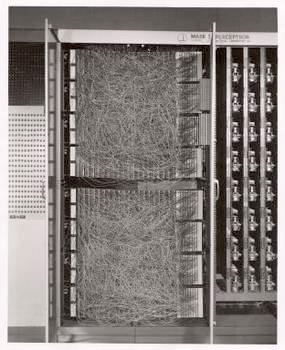
\includegraphics[width=.45\textwidth]{figures_c3/mlpregressor/Mark_I_perceptron.jpg}
        \caption{\textbf{The Mark 1 perceptron} Both software and hardware are different manifestations of a flow chart. The perceptron hardware accomplished what is now done using software. Source: \cite{perceptronimage}}
        \label{fig:perceptron}
\end{figure}

\subsubsection{The Multi-Layer Perceptron}\label{sec:perceptron}
Limitations of the perceptron include the classification of complex patterns such as the XOR problem (where a category appears between two other categories e.g. {1|0|1} - this cannot be classified by a single linear split). In taking inspiration from nature, \autoref{fig:layercortex}, it is possible to overcome this with the use of multiple layers. This creates a deep ($>2$ two hidden (non-input) layers of perceptrons\footnote{These are sometimes referred to as Linear Threshold Units.}) artificial neural network (ANN) 

The multi-layer perceptron (MLP) model now represents a simple feed-forward network, much like a decision tree. However, unlike a decision tree, the MLP ANN can describe the probability a branch is taken using non-linear activation (threshold) functions. These are discussed in detail as part of \autoref{sec:ae}. The weighting thresholds for each neuron are then calculated by backwards propagation of results through the network until a suitably good result is produced. 

\begin{quote}
\textit{
\textbf{Example analogy:} Backpropagation can be likened to the iterative calibration of scientific instrumentation. In the field of atmospheric chemistry, laser-induced fluorescence is used to calculate species concentrations and reaction rates within the troposphere, \citep{lif1,lif2}. Here the frequency of a laser can be adjusted in contrast with a known target (e.g. an amount of \ce{SO2}) to produce a response curve showing where the maximum resonance occurs.\\
Similarly, a neural network can be `trained' (calibrated). 
This is done through the use of a `training dataset' - a set of input-output pairings which represent a random selection of 2/3rds of the total dataset. Next, the neurons within each layer (similar to the potentiometer dials on an instrument) are adjusted in sequence through the layers to match the known result (a standard of known concentration) to the input values provided. This process is repeated until for many iterations, or until a sufficiently `good' prediction is attained for the entire training dataset (early termination). The power of ANNs comes from the ability to adjust neuron thresholds whilst moving both forwards and backwards through the network (Note: predictions of an MLP are still only passed forwards). Finally, model performance is evaluated against the remaining 1/3rd of the total dataset.
}
\end{quote}


\begin{figure}[H]
     \centering
         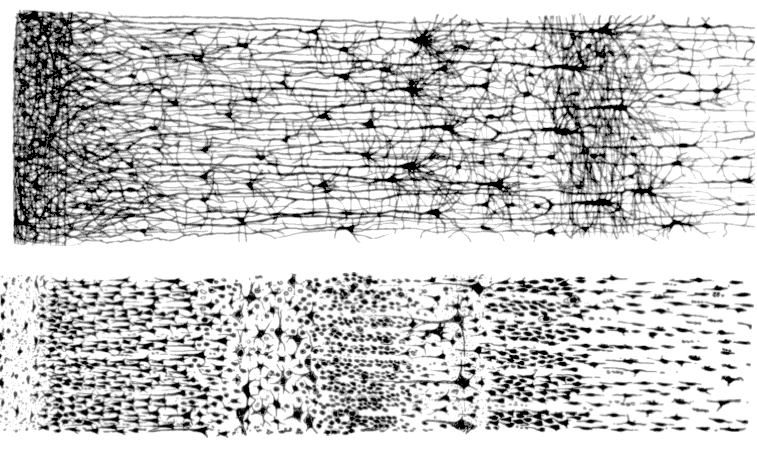
\includegraphics[width=.85\textwidth]{figures_c3/mlpregressor/Cajal_cortex_drawings.png}
        \caption{\textbf{The Human Cortex - A biological neural network.}. A vertical cross section of the human cortex between an adult (top) and 1.5 month old infant (bottom) showing a layer like structure with a change in depth (left to right). Source: \cite{layercortex}}
        \label{fig:layercortex}
\end{figure}

\subsubsection{Applying the MLPRegressor to Observational data}
In the application of any type of machine aided algorithms, it is important to evaluate the results provided. In this section, the results of 12 years of data collected as part of the [CAPE VERDE CAMPAIGN] are shown (these contain measurements spanning the entirety of 12 years, which produce the clearest tests for the algorithm). A MLPRegressor of 10 hidden layers, and a hyperbolic tan (tanh) activation function is used \autoref{sec:appendix:tanh}. Additionally, the limited-memory Broyden–Fletcher–Goldfarb–Shanno (l-BFGS) solver (a quasi-newton method which minimises the inverse of the Hessian matrix\footnote{ The hessian is square matrix of second-order partial derivatives of a scalar-valued function/field describing the local curvature of a function (of many variables).} to steer through space and obtain a solution) and an adaptive learning rate\footnote{Each time the model improvement fails to decrease the learning loss, the learning rate is reduced by 1/5. This means smaller jumps are made towards the curve peak. } is used. 

The input of the regressor is in the form of a month and an hour, to represent each measurement. This allows it to find not only daily trends but also seasonal trends within the data. Once trained the regressor is then used to predict a diurnal profile for each month based on the observational data provided. For simplicity $\log_{10}$ values of the concentrations obtained have been used. To validate the results, the predicted MLPRegressor line is compared to a transparent scatterplot for all the results. In addition to this, a boxplot showing the IQR, median and mean (green line) plotted alongside to evaluate the predictor output. 

In providing the MLPRegressor with both month and hour inputs, the data is not only fitted hourly (a diurnal average) but also across the seasonal/monthly cycles. This accounts for the variation between years and datasets. Since $\log_{10}$ values of the concentrations are used, species such as ozone (\autoref{fig:mlpo3}) which for the Cape Verde dataset (clean air) do not change more than one order of magnitude, the effects of neighbouring months, which shift the diurnal away from the mean (the green line on the boxplot), can be seen. However since this is overall a small change, and the diurnals lie within the interquartile range, they still provide an adequate approximation. NO (\autoref{fig:mlpno}) on the other hand has a concentration change of several orders of magnitude. Here a distinct daytime peak is seen and is centred around a seasonally consistent mean value of the data. Here the multi-magnitude change in concentration also provides an effective silhouette of the data to which we may compare the fitted line. 
Finally the plots of \ce{NO2} and iso-Pentane (\autoref{fig:mlpno2}-\ref{fig:mlpisopentane}) vary both in diurnal magnitude and seasonally. Within these plots, changes in the data in the January and December months produce deceptively misleading results. Here although the diurnals are not symmetric, they fit well within the median, mean and interquartile range values, as well as the general data silhouette behind them. This suggests that it is a property of the data that we are fitting, and not that the regressor is producing incorrect results. It is however noted that for a more accurate seasonal prediction, periodic boundary conditions should be employed in the training dataset, where an additional two months are added before January and after December. As only a single value estimate from the summer region will be taken, this does not affect the result accuracy. 

\begin{figure}[H]
     \centering
         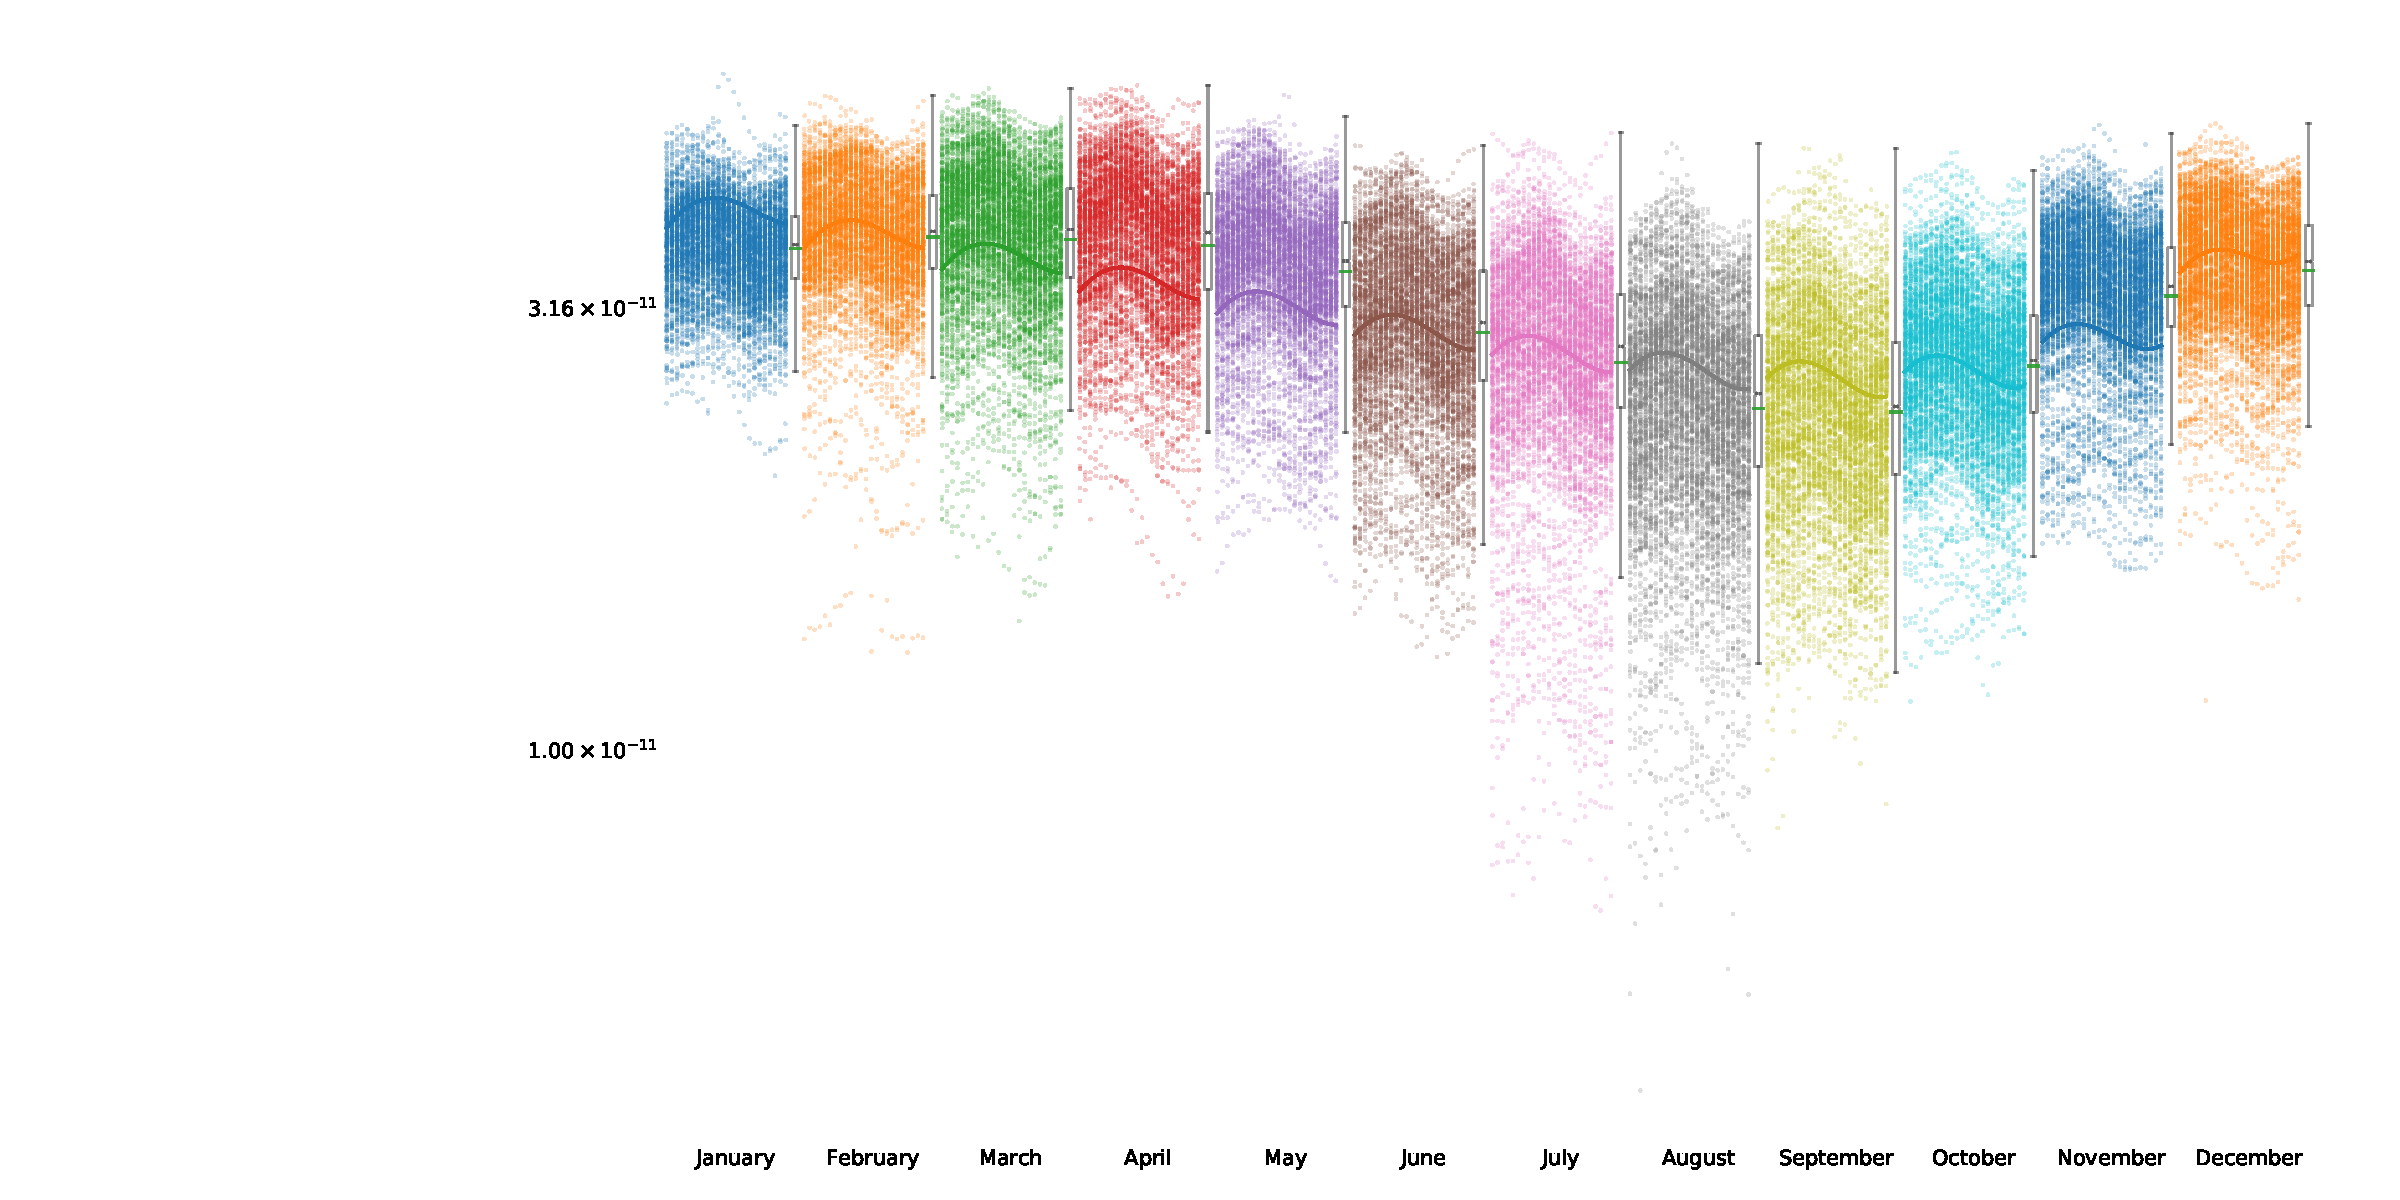
\includegraphics[width=.90\textheight,angle =90,trim={8cm 0 0 0}]{figures_c3/mlpregressor/CVNOX_CapeVerde/O3.pdf}
        \caption{\textbf{Cape Verde MLP predicted and observational data of Ozone.} Each segment represents data from a different month. Within each month segment exists 24 hour segments to create a diurnal. Observational concentrations are plotted in the form of a translucent scatterplot and summarised using the boxplot on the right of the month segment. MLP predicted results are shown using the solid lines. Concentration in mixing ratio.}
        \label{fig:mlpo3}
\end{figure}

\begin{figure}[H]
     \centering
         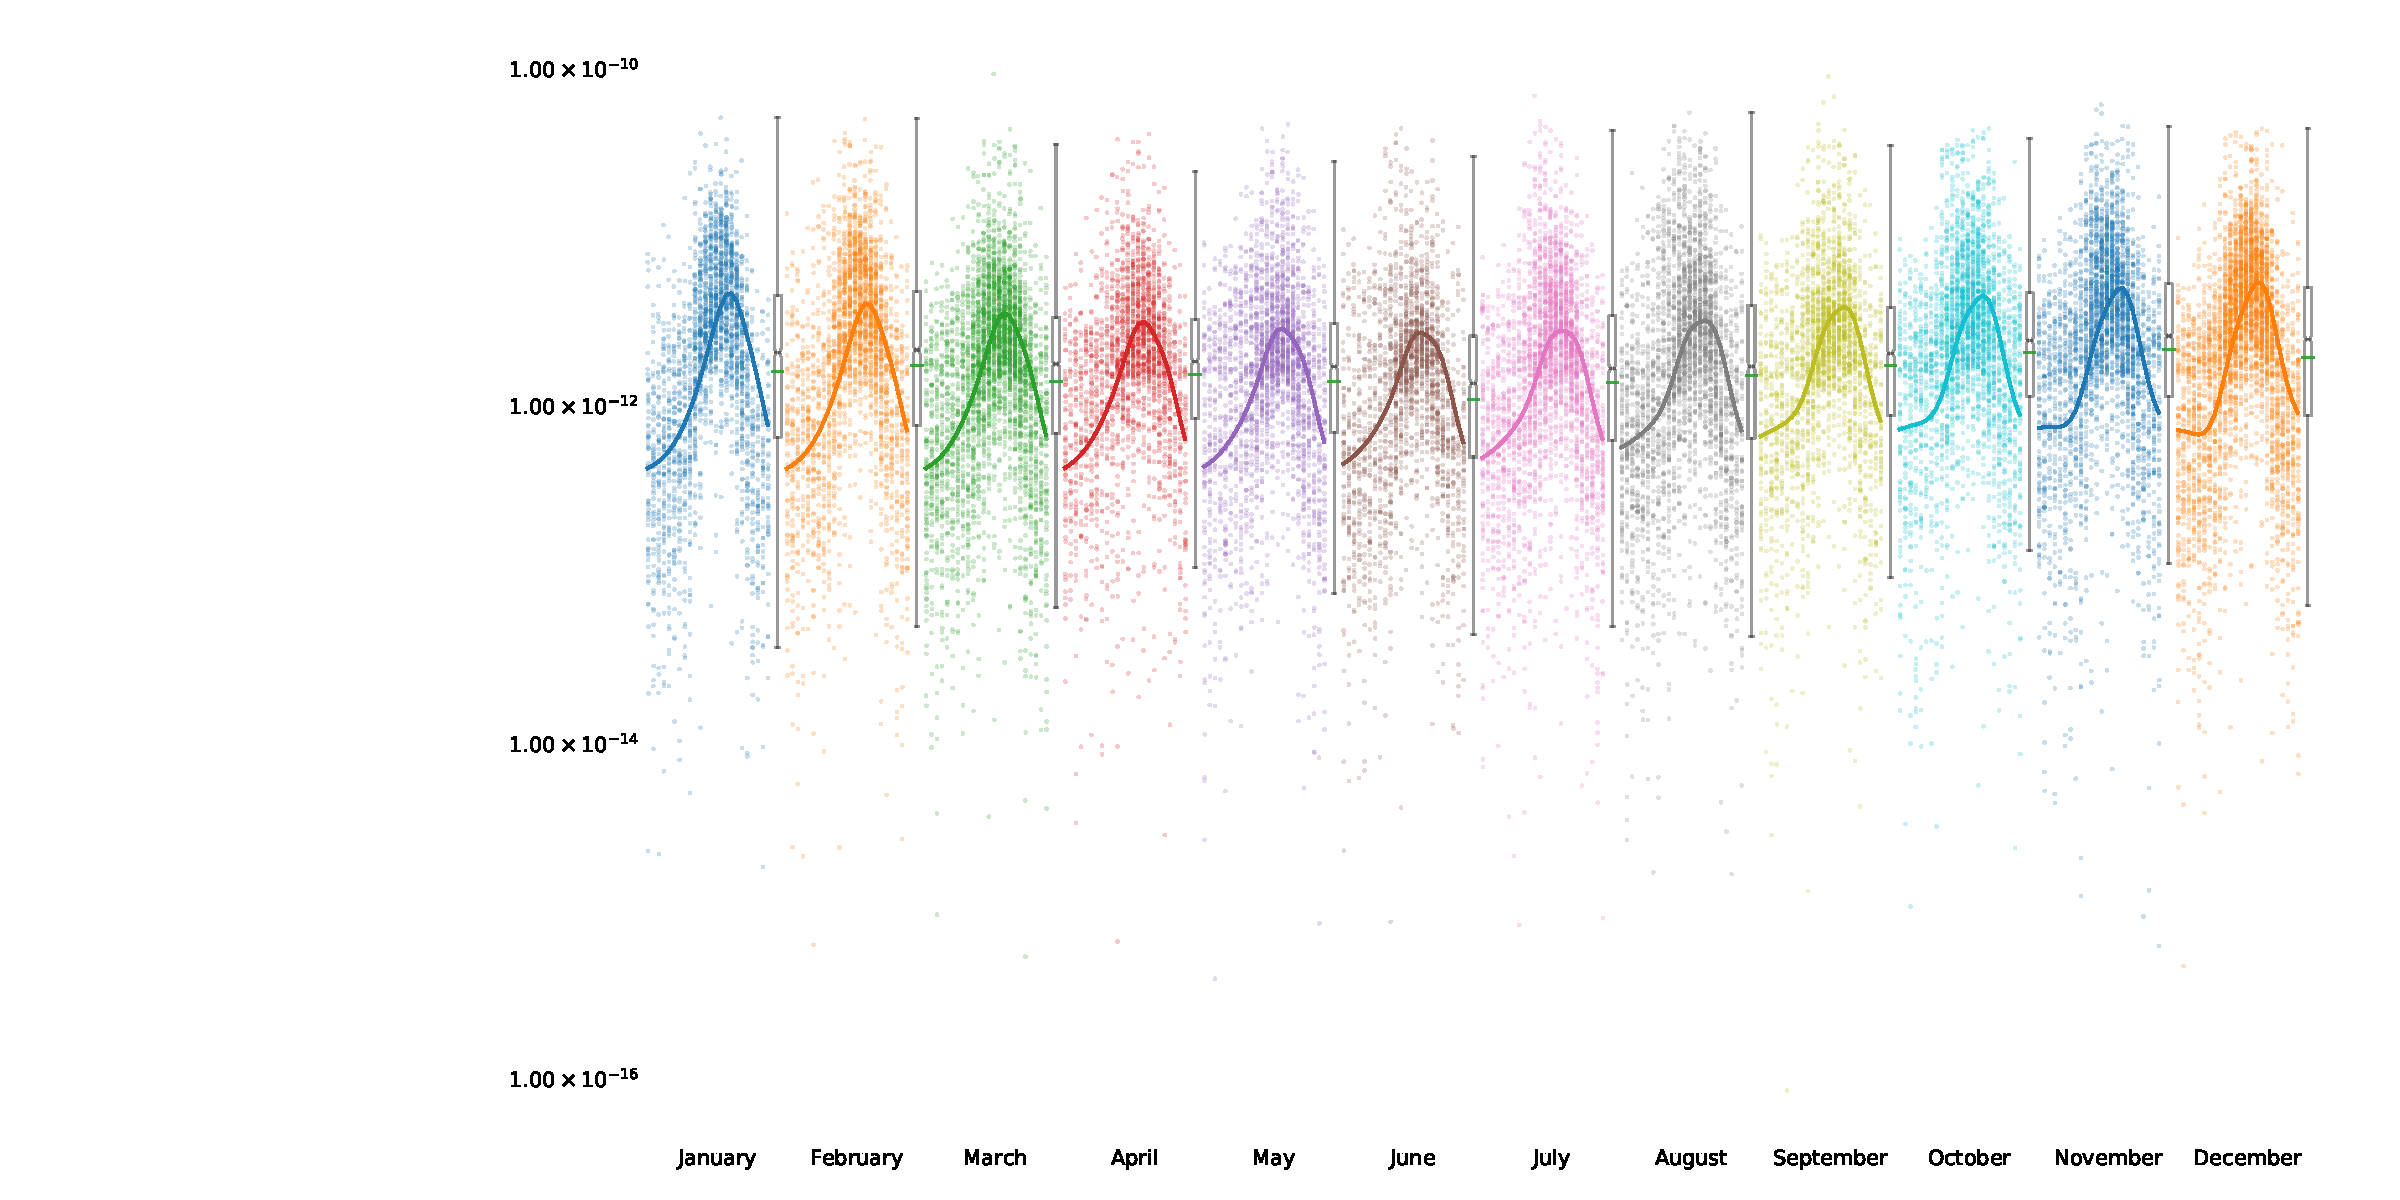
\includegraphics[width=.90\textheight,angle =90,trim={8cm 0 0 0}]{figures_c3/mlpregressor/CVNOX_CapeVerde/NO.pdf}
        \caption{\textbf{Cape Verde MLP predicted and observational data of NO.} Each segment represents data from a different month. Within each month segment exists 24 hour segments to create a diurnal. Observational concentrations are plotted in the form of a translucent scatterplot and summarised using the boxplot on the right of the month segment. MLP predicted results are shown using the solid lines. Concentration in mixing ratio.}
        \label{fig:mlpno}
\end{figure}

\begin{figure}[H]
     \centering
         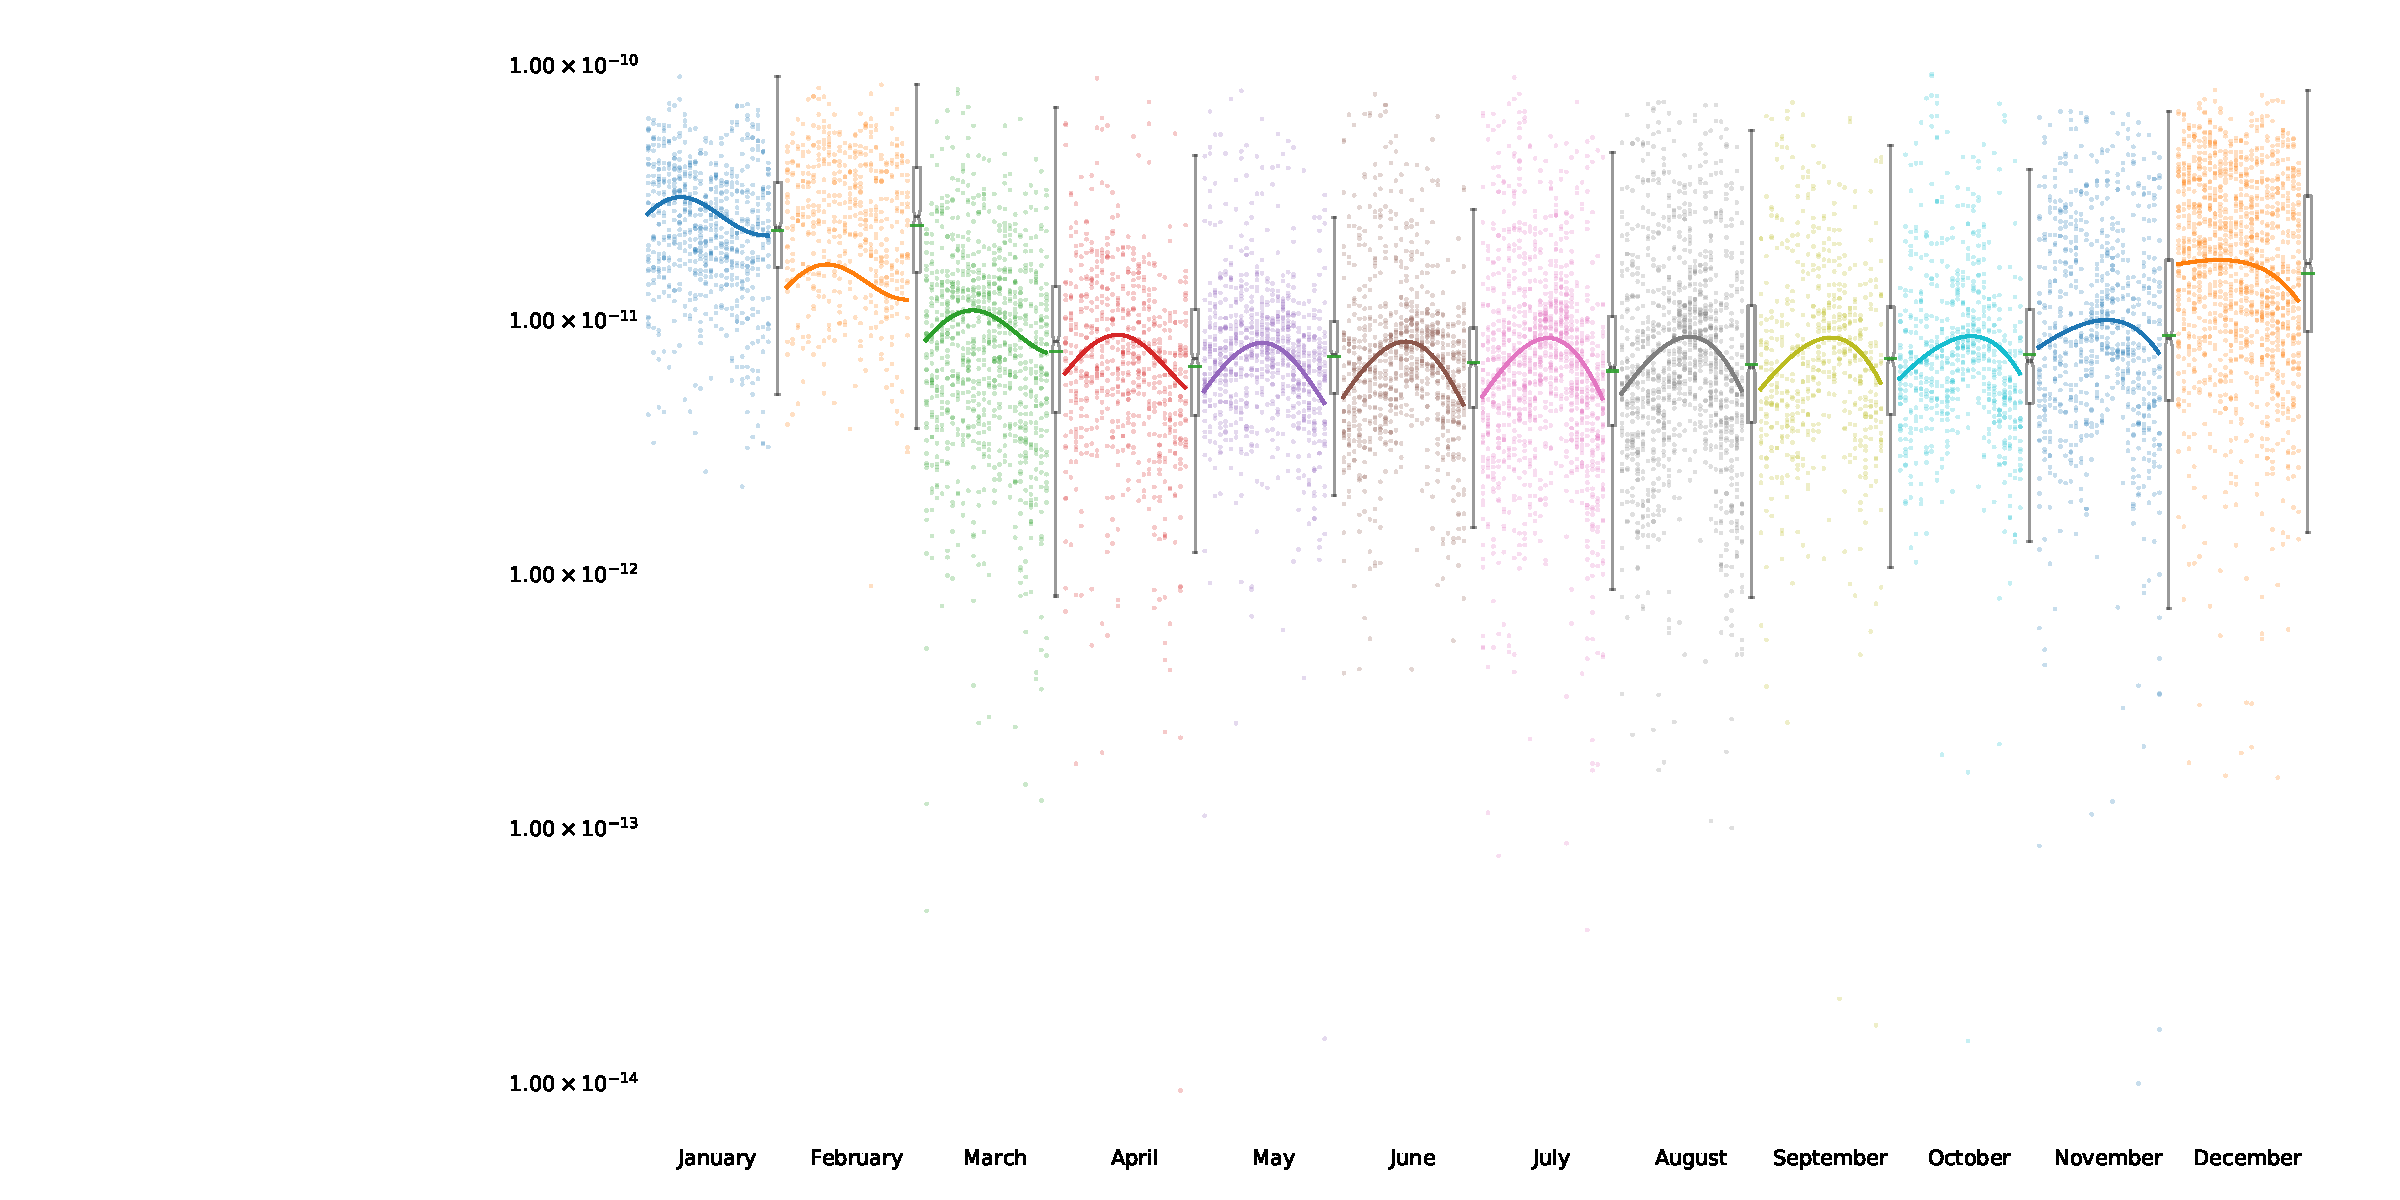
\includegraphics[width=.90\textheight,angle =90,trim={8cm 0 0 0}]{figures_c3/mlpregressor/CVNOX_CapeVerde/NO2.pdf}
        \caption{\textbf{Cape Verde MLP predicted and observational data of \ch{no2}.} Each segment represents data from a different month. Within each month segment exists 24 hour segments to create a diurnal. Observational concentrations are plotted in the form of a translucent scatterplot and summarised using the boxplot on the right of the month segment. MLP predicted results are shown using the solid lines. Concentration in mixing ratio.}
        \label{fig:mlpno2}
\end{figure}

\begin{figure}[H]
     \centering
         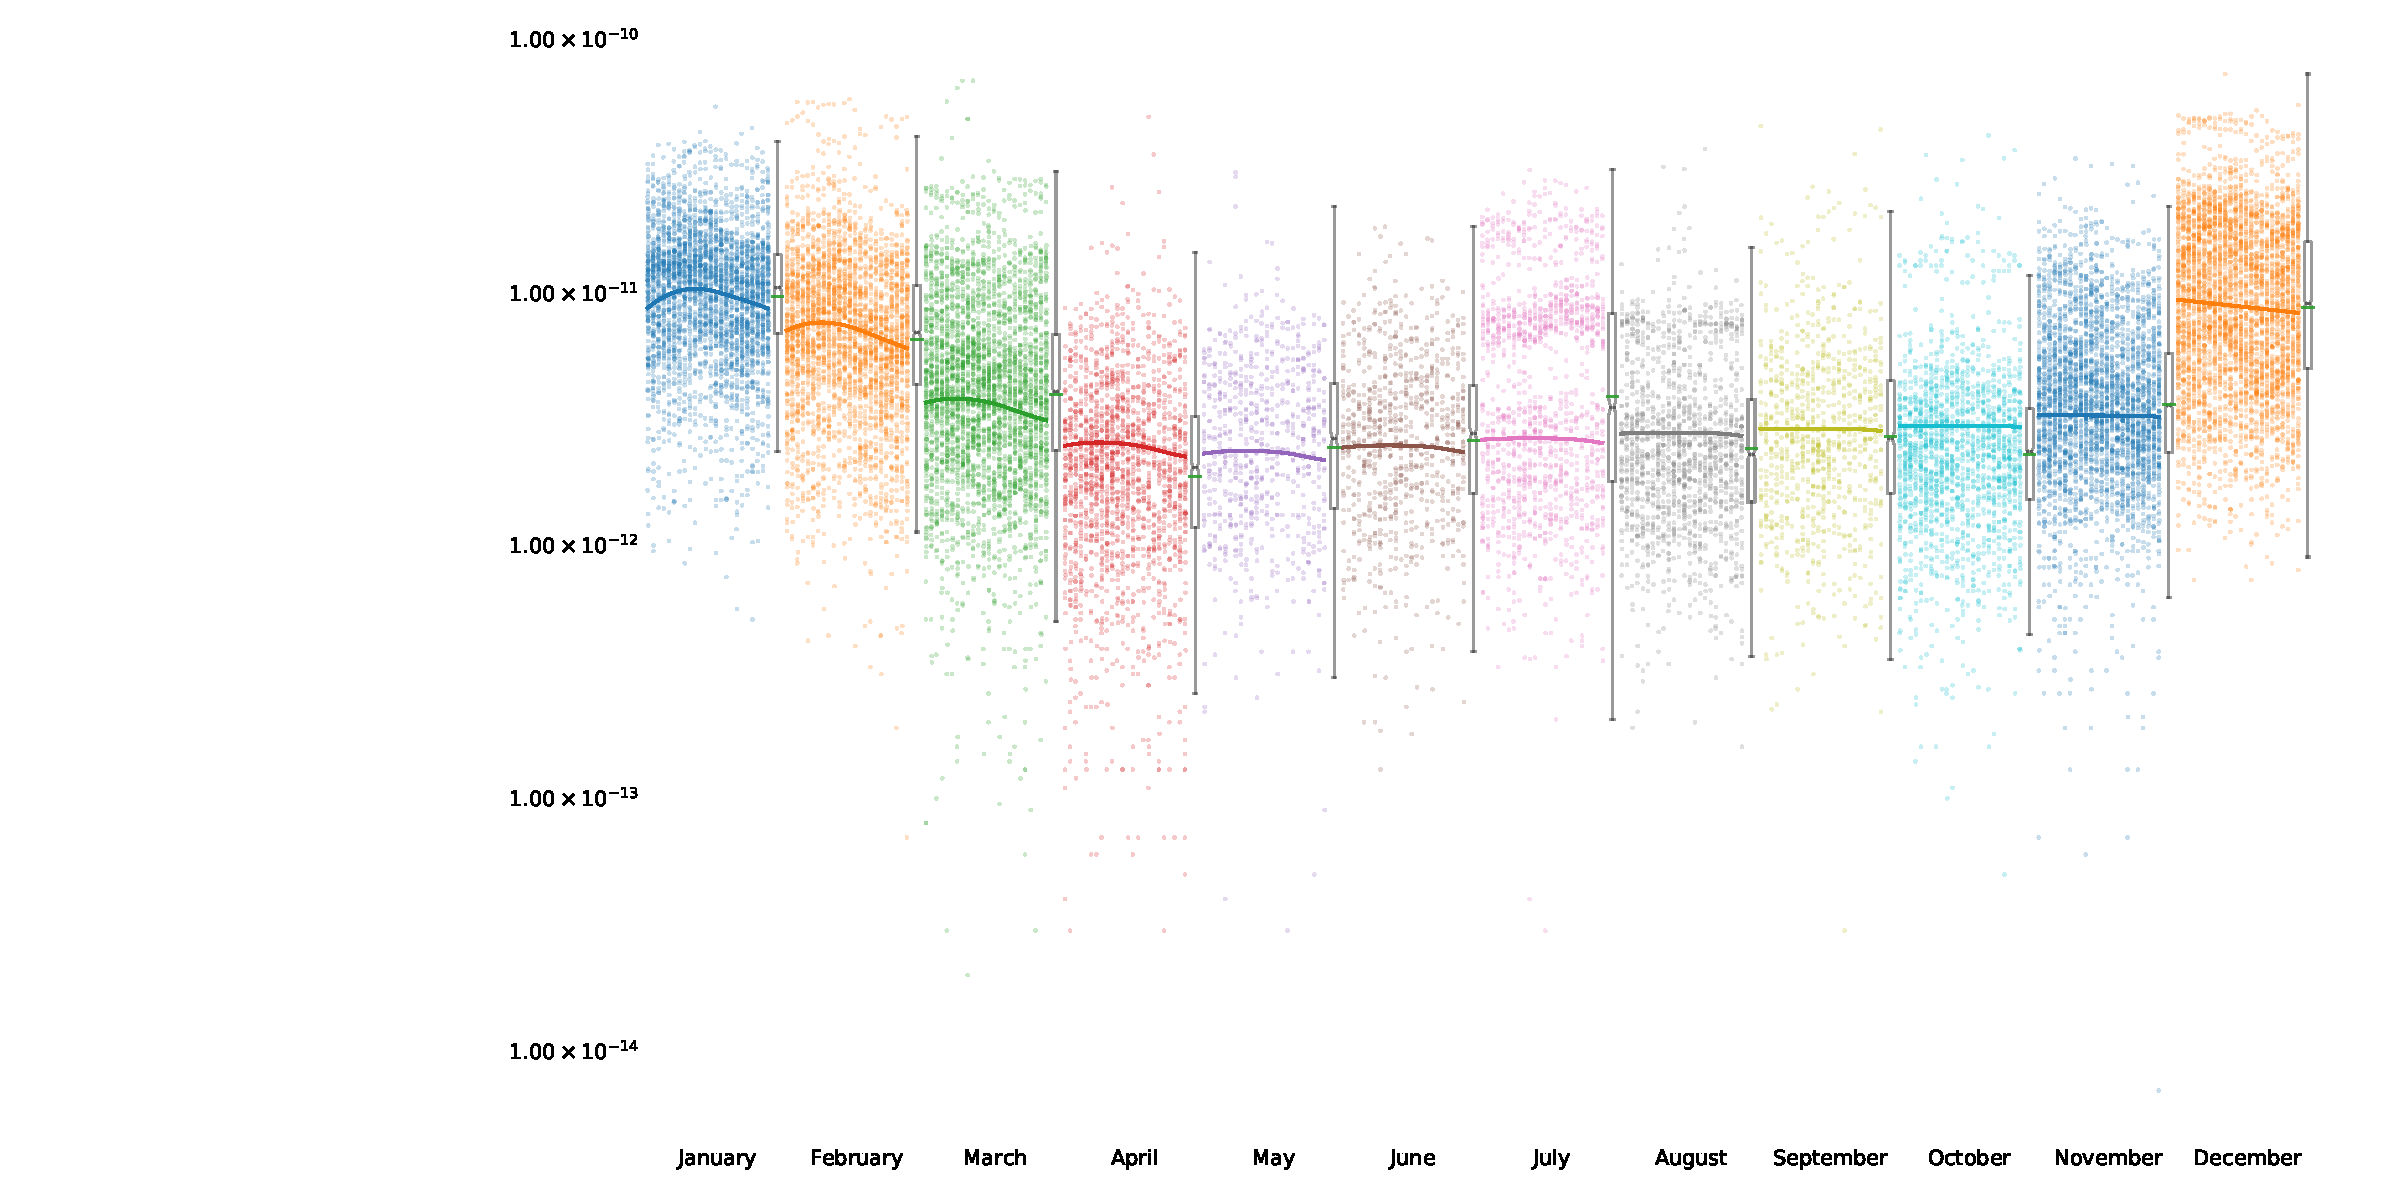
\includegraphics[width=.90\textheight,angle =90,trim={8cm 0 0 0}]{figures_c3/mlpregressor/CVNOX_CapeVerde/ISO_PENTANE.pdf}
        \caption{\textbf{Cape Verde MLP predicted and observational data of iso-Pentane.} Each segment represents data from a different month. Within each month segment exists 24 hour segments to create a diurnal. Observational concentrations are plotted in the form of a translucent scatterplot and summarised using the boxplot on the right of the month segment. MLP predicted results are shown using the solid lines. Concentration in mixing ratio. }
        \label{fig:mlpisopentane}
\end{figure}


\subsubsection{Model Initialisation Procedure}
The aim is to generate a set of initiation concentrations which are representative of the different types of chemistry between environments. In this section, we are not interested in the exact concentration modelling for specific times or scenarios. Instead, we seek to generate representative of the processed chemistry under a range of conditions. 

To do this species concentrations are extracted from an MLP regressor trained on observational data for each scenario. Each concentration is that of noon local time from the generated diurnal from summer observations at each location. This produces a monthly error of $\pm 2 months$ from June. As both nitrogen oxide and dioxide are supplied the total NO$_x$ for each simulation are \emph{not} constrained. The initial conditions are shown in \autoref{tab:icsmetric}.

In general observational measurements are not able to detect all the species presented within the MCM. This means that to be able to compare model scenarios, the chemistry must first be spun up. In propagating the chemistry forwards in time, primarily emitted and measured species are broken up forming the intermediate species which exist within a mechanism. To reach a steady-state, the model is initiated at noon and the observational concentrations are rest every 24 hours. For each diurnal, the fractional difference between the concentrations at each day are compared. If the difference between these is less than 0.001, the model is left to run unconstrained for 5 days (right of the dashed line in \multiref{fig:ccape}{fig:cbeijing}). Model results are then taken after 3 days of unconstrained runs. The reason for this is that the total RO$_2$ concentration takes longer to stabilise in the polluted environments (London and Beijing). This falls into a periodic cycle beginning noon on the third day and can provide a representation of the processed chemistry within each environment. 

\textit{NOTE: It should be noted that some of the concentration plots may appear to lose their diurnal dependability. This may be attributed to the changing order of magnitude of the concentrations, and that the species are still responding as expected. }

\subsubsection{Extracting the required results}
Model diagnostics such as concentration and the net flux passing through a species may be extracted directly from the DSMACC box model. These provide the baseline comparison and can be directly compared to the graph metrics. Species concentration tells us the abundance of different species, and the net-flux tells us how fast this is changing in time. 

As some species may have a fast inwards and outwards flux (low net-flux), the absolute flux is also included. Finally, the sensitivity of each species for other species is also extracted (the jacobian matrix). This serves to not only generate the graph used to represent the chemistry, (\autoref{sec:graphconstruction}) but also to identify the overall influence a species has on others in the network. This can be calculated by taking the net sum of the influence a species has on every other from the Jacobian. This is analogous to calculating the outdegree of a node in the jacobian network. 
\newpage
 
\begin{table}[H]
\centering
\small


\begin{table}[H]
\centering
\small

%%%%%%%
\begin{tabular}{p{0.2\textwidth}p{0.16\textwidth}p{0.16\textwidth}p{0.16\textwidth}p{0.16\textwidth}}
\toprule
Species & Beijing(APHH) & Borneo(OP3) &  London(ClearFlo) &  CapeVerde \\
\midrule
\ce{LAT}       & 39.9 &              0.96 &            51.0&       16.5 \\
\ce{LON}       &  116.3 &              114.5 &            0.00 &       23.4 \\
\midrule
CO & 3.829e-06 & 3.321e-07& 7.780e-09 & 0.0*\\
\ce{O3}        &  6.883e-08 &              8.939e-09 &            3.819e-08 &       2.629e-11* \\
\ce{NO}        &  1.660e-09 &              2.668e-14* &            2.350e-09 &       2.358e-12 \\
\ce{NO2}       &  1.226e-08 &              1.081e-13* &            7.445e-09 &       8.447e-12 \\
\ce{HCHO}      &  4.472e-09 &                        &            1.119e-08 &                 \\
\ce{C2H6}      &  3.163e-09 &              7.315e-10 &            2.133e-09 &       4.539e-10 \\
\ce{C2H4}      &  1.004e-09 &              1.152e-10 &            4.893e-10 &       2.481e-11 \\
\ce{C3H8}      &  3.019e-09 &              1.924e-10 &            1.128e-09 &       1.728e-11 \\
\ce{C3H6}      &  1.335e-10 &              1.333e-11 &            1.784e-10 &       9.343e-12 \\
\ce{IC4H10}    &  6.412e-10 &              8.742e-11 &            5.142e-10 &       2.486e-12 \\
\ce{NC4H10}    &  1.593e-09 &              5.698e-11 &            1.058e-09 &       4.481e-12 \\
\ce{C2H2}      &  1.058e-09 &              1.825e-10 &            3.018e-10 &       1.848e-11 \\
{TBUT2ENE}  &  4.198e-11 &                        &            1.815e-11 &                 \\
{CBUT2ENE}  &  4.454e-11 &                        &            1.305e-11 &                 \\
\ce{IC5H12}    &  1.047e-09 &              2.883e-11 &            7.424e-10 &       3.470e-12 \\
\ce{NC5H12}    &  4.650e-10 &              2.090e-11 &            2.792e-10 &       2.513e-12 \\
{TPENT2ENE} &  3.939e-11 &                        &                      &                 \\
{CPENT2ENE} &  3.982e-11 &                        &                      &                 \\
\ce{NC6H14}    &  2.057e-10 &              6.437e-12 &            6.357e-11 &                 \\
\ce{C5H8}      &  7.134e-10 &              1.957e-09 &            1.640e-10 &                 \\
\ce{NC7H16}    &  7.905e-11 &                        &            5.222e-11 &                 \\
\ce{BENZENE}   &  4.045e-10 &                        &            1.137e-10 &       7.682e-12 \\
\ce{NC8H18}    &  3.091e-11 &                        &            1.442e-11 &                 \\
\ce{TOLUENE}   &  6.767e-10 &                        &            3.205e-10 &       3.121e-12 \\
\ce{EBENZ}     &  3.115e-10 &                        &            6.017e-11 &                 \\
\ce{OXYL}      &  1.677e-10 &                        &            5.049e-11 &                 \\
\ce{CH3CHO}    &  4.783e-10 &                        &            4.095e-09 &                 \\
\ce{C2H5OH}    &  4.655e-09 &                        &            3.125e-09 &                 \\
\ce{CH3COCH3}  &  3.328e-09 &                        &            2.924e-09 &                 \\
\ce{NC9H20}    &  1.336e-11 &                        &            7.922e-11 &                 \\
\ce{NC10H22}   &  1.062e-12 &                        &            1.602e-10 &                 \\
$\alpha$-\ce{PINENE}\footnotemark
   &  7.341e-11 &     15e-11                   &            1.105e-10 &                 \\
\ce{LIMONENE}  &  5.836e-11 &              1.351e-10 &            3.566e-11 &                 \\
\ce{PXYL+MXYL}\footnotemark
 &  4.943e-10 &                        &                      &                 \\
\ce{IPBENZ}    &  4.567e-10 &                        &                      &                 \\
\ce{PBENZ}     &  3.996e-10 &                        &                      &                 \\
\ce{HONO}      &  6.479e-10 &                        &            4.109e-10 &                 \\
\ce{MACR}      &            &              6.948e-11 &            1.862e-11 &                 \\

%%%%%%%%%%%%%%%
\bottomrule
\end{tabular}
\end{table}


\begin{table}[H]
\centering
\small
\begin{tabular}{p{0.2\textwidth}p{0.16\textwidth}p{0.16\textwidth}p{0.16\textwidth}p{0.16\textwidth}}
\toprule
Species & Beijing(APHH) & Borneo(OP3) &  London(ClearFlo) &  CapeVerde \\
\midrule

%%%%%%%%%%%%%%

{PENT1ENE}  &            &                        &            2.383e-11 &                 \\
\ce{MVK}       &            &                        &            2.091e-11 &                 \\
\ce{NPROPOL}   &            &                        &            2.883e-10 &                 \\
\ce{NBUTOL}    &            &                        &            4.535e-10 &                 \\
\ce{STYRENE}   &            &                        &            2.241e-11 &                 \\
\ce{MEK}       &            &                        &            5.494e-11 &                 \\
\ce{C3H7CHO}   &            &                        &            9.534e-12 &                 \\
\ce{C4H9CHO}   &            &                        &            1.865e-11 &                 \\
\ce{C5H11CHO}  &            &                        &            1.201e-11 &                 \\
\ce{CYHEXONE}  &            &                        &            9.790e-12 &                 \\
\ce{BENZAL}    &            &                        &            1.510e-11 &                 \\
\ce{PAN}       &            &                        &            1.791e-10 &                 \\
\bottomrule
\end{tabular}


\caption{(2-page split) The initial conditions created from the MLPRegressor prediction of observational data. Although not specified the mixing ratios for methane is set by the model at 1770ppb, the temperature is 298K, and water vapour is at 2\%. \textbf{* Starred values are of the wrong units and should be multiplied by 1000. As there was no time to rerun these, their results have been omitted from this chapter.}}
\label{tab:icsmetric}
\end{table}

\footnotetext{This is (incorrectly) written as `?-pinene' in the merged CEDA dataset for the Borneo OP3 campaign. This is due to character conversion errors.}
\footnotetext{The mixing ratios for these is split evenly between both species}

\caption{The initial conditions created from the MLPRegressor prediction of observational data. Although not specified the concentration for methane is set by the model at 1770ppb.}
\label{tab:icsmetric}
\end{table}

\footnotetext{This is written as ?-pinene in the merged CEDA dataset for the Borneo OP3 campaign. This is due to character conversion errors.}
\footnotetext{The concentration for these is split evenly between both species}
\newpage


\begin{figure}[H]
    \centering
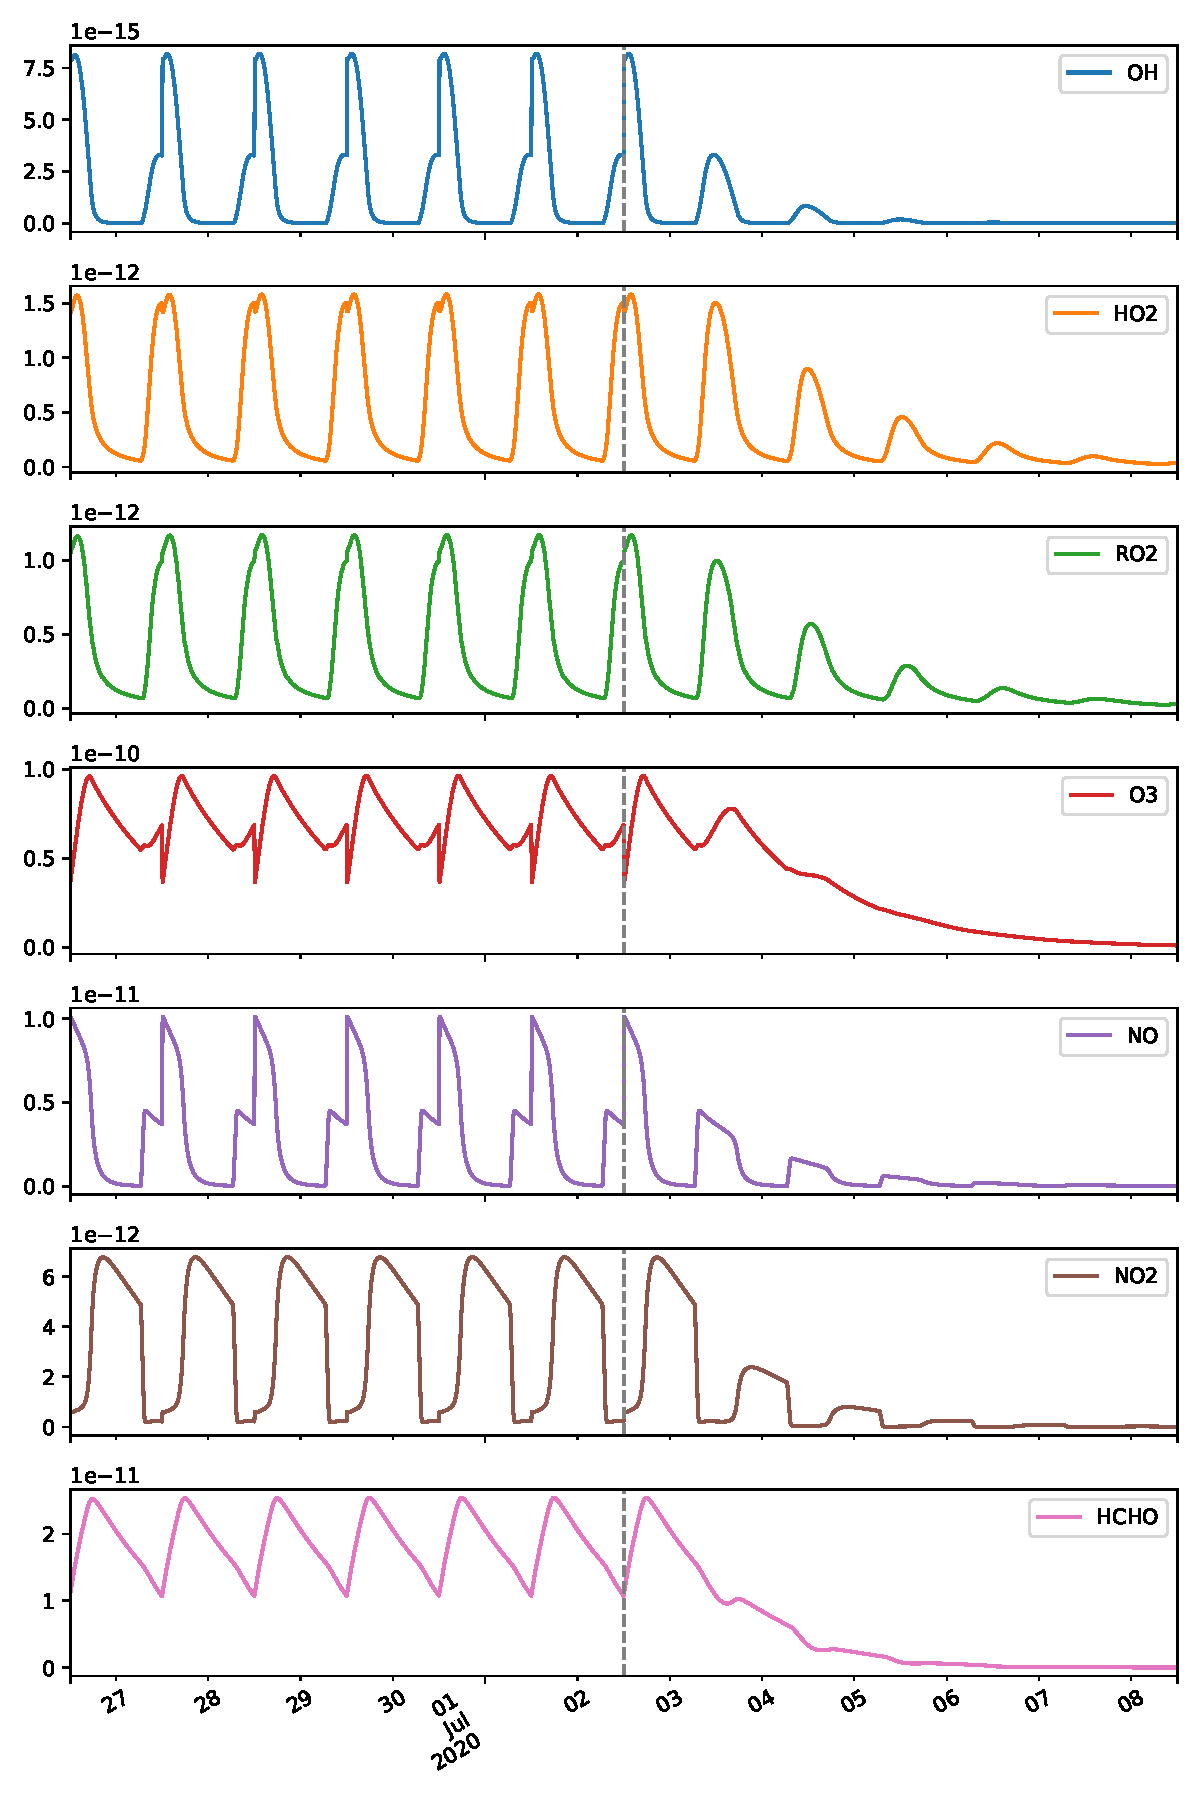
\includegraphics[width=.9\textwidth]{figures_c3/mlpregressor/conc_cape.pdf}
\caption{\textbf{The concentration profile for CapeVerde.}This shows a the change in concentration over time for HO$_x$,NO$_x$,Ozone and RO$_2$ species for a simulation run generated by the mlpregressor. Left of the dashed line shows the last 6 days of spinup, where the intial concentrations are reset at noon each day until the species fractional difference is less than 0.001 .}
\label{fig:ccape}
\end{figure}

\newpage


\begin{figure}[H]
    \centering
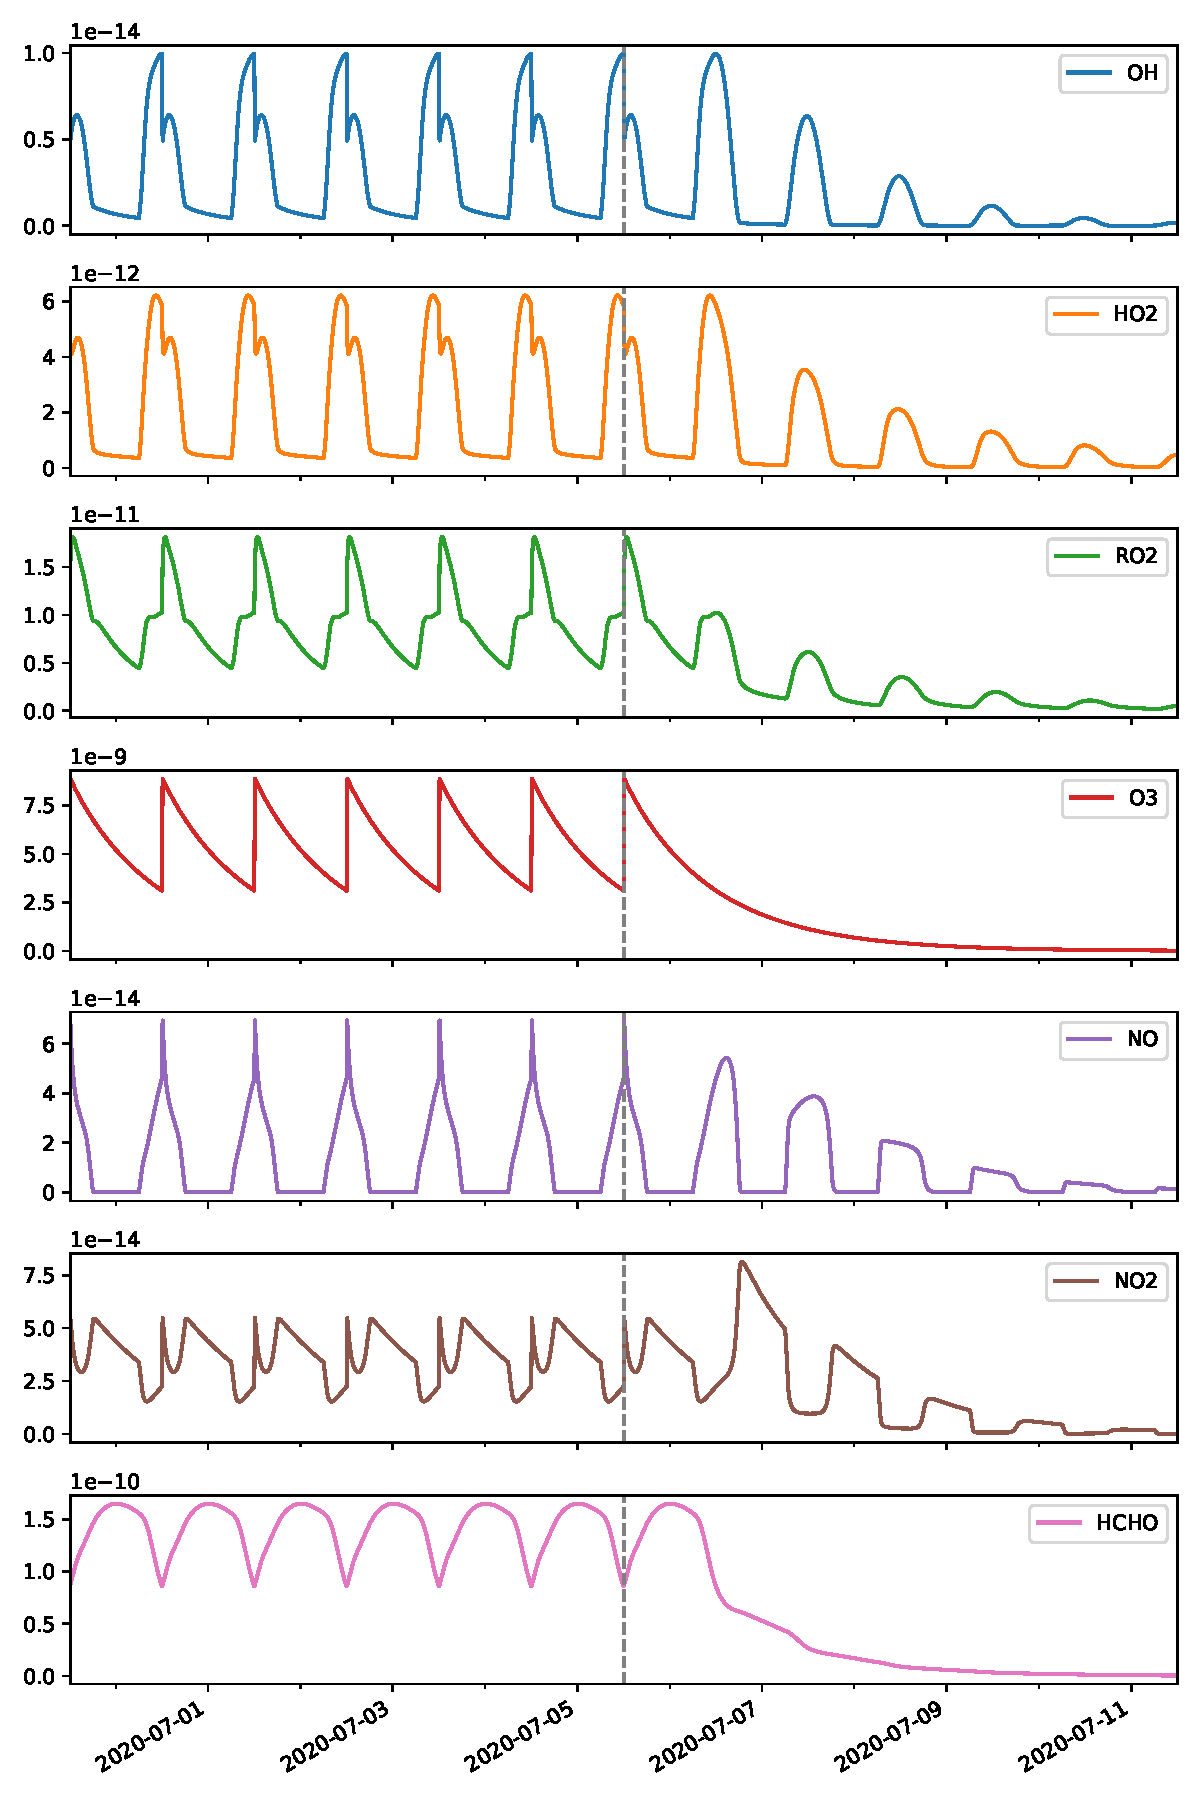
\includegraphics[width=.9\textwidth]{figures_c3/mlpregressor/conc_borneo.pdf}

\caption{\textbf{The concentration profile for Borneo.}This shows a the change in concentration over time for HO$_x$, NO$_x$, Ozone and RO$_2$ species for a simulation run generated by the MLPRegressor. Left of the dashed line shows the last 6 days of spinup, where the initial concentrations are reset at noon each day until the species fractional difference is less than 0.001 .}
\label{fig:cborneo}
\end{figure}

\newpage


\begin{figure}[H]
    \centering
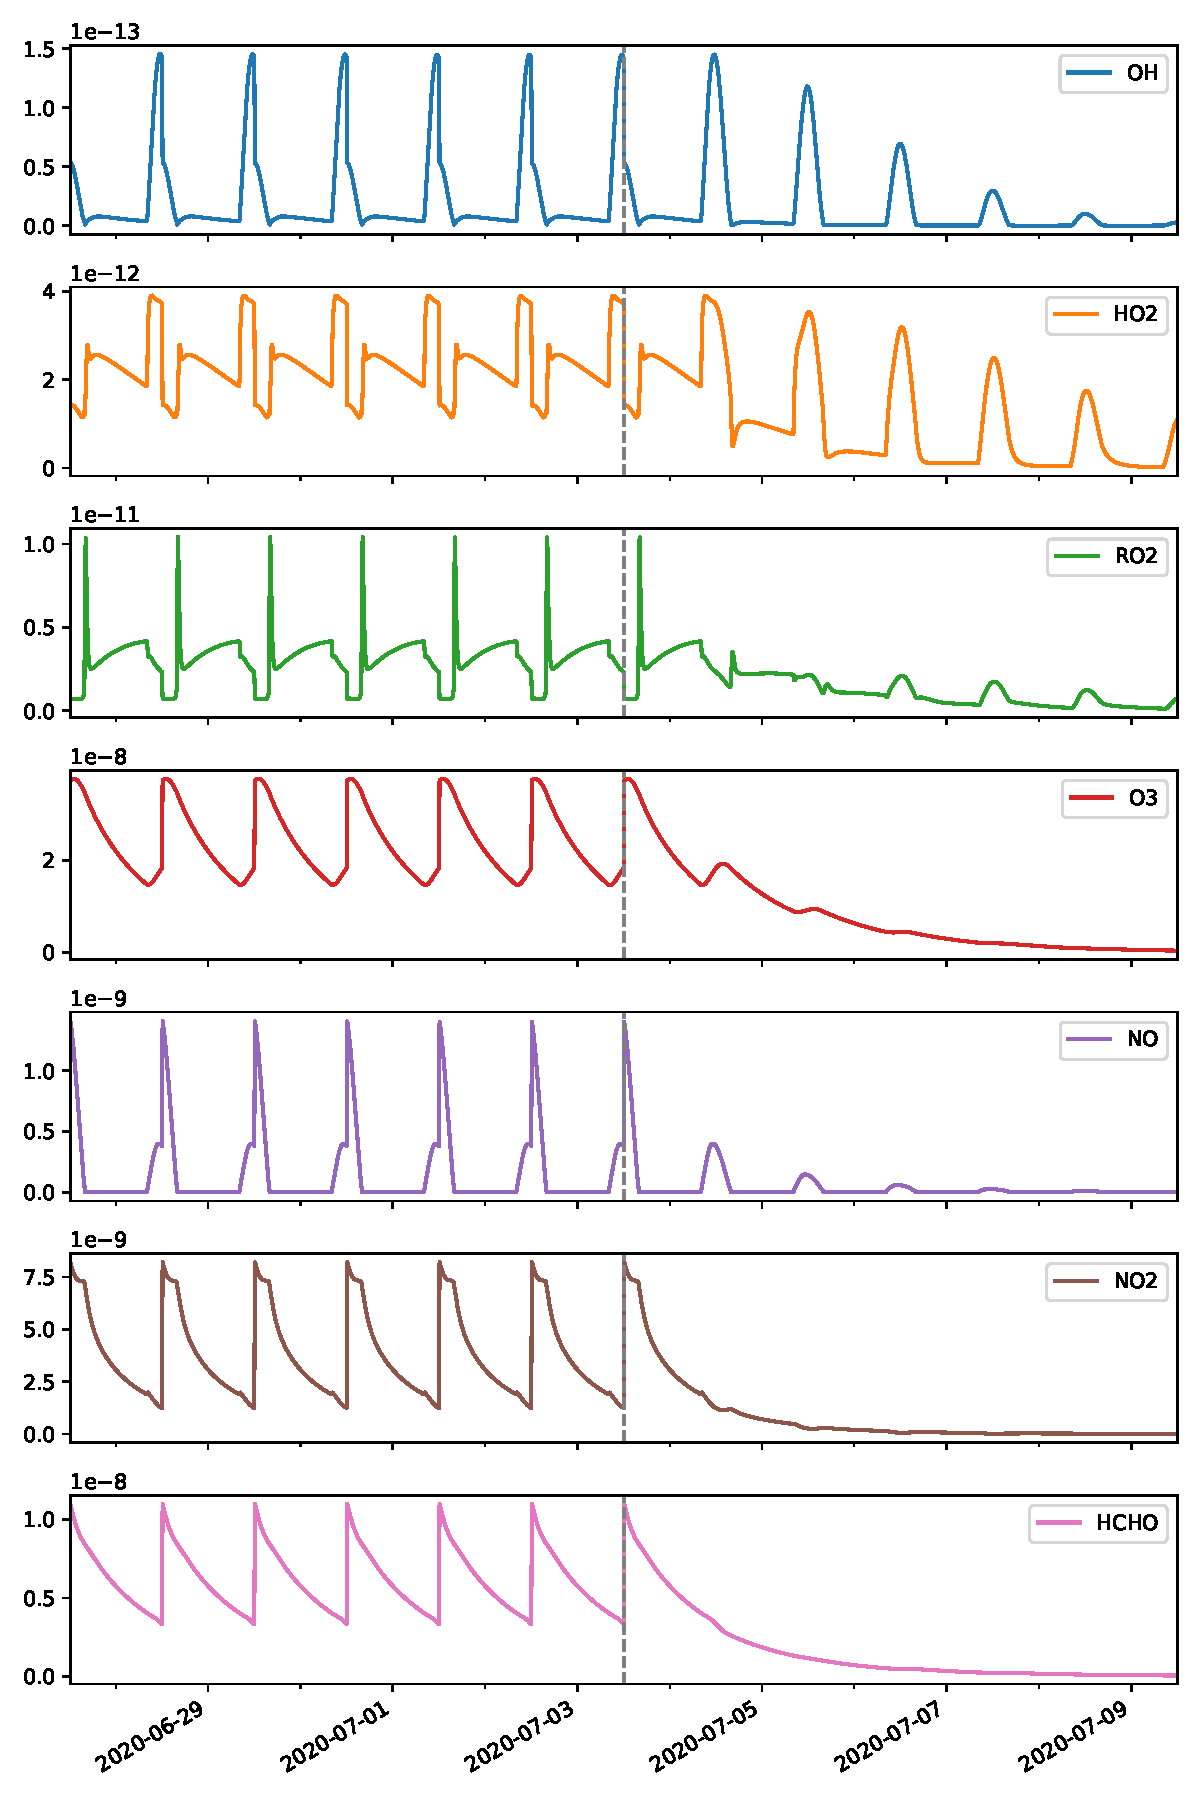
\includegraphics[width=.9\textwidth]{figures_c3/mlpregressor/conc_clfo.pdf}
\caption{\textbf{The concentration profile for London.}This shows a the change in concentration over time for HO$_x$,NO$_x$,Ozone and RO$_2$ species for a simulation run generated by the mlpregressor. Left of the dashed line shows the last 6 days of spinup, where the intial concentrations are reset at noon each day until the species fractional difference is less than 0.001 .}
\label{fig:clondon}
\end{figure}

\newpage


\begin{figure}[H]
    \centering
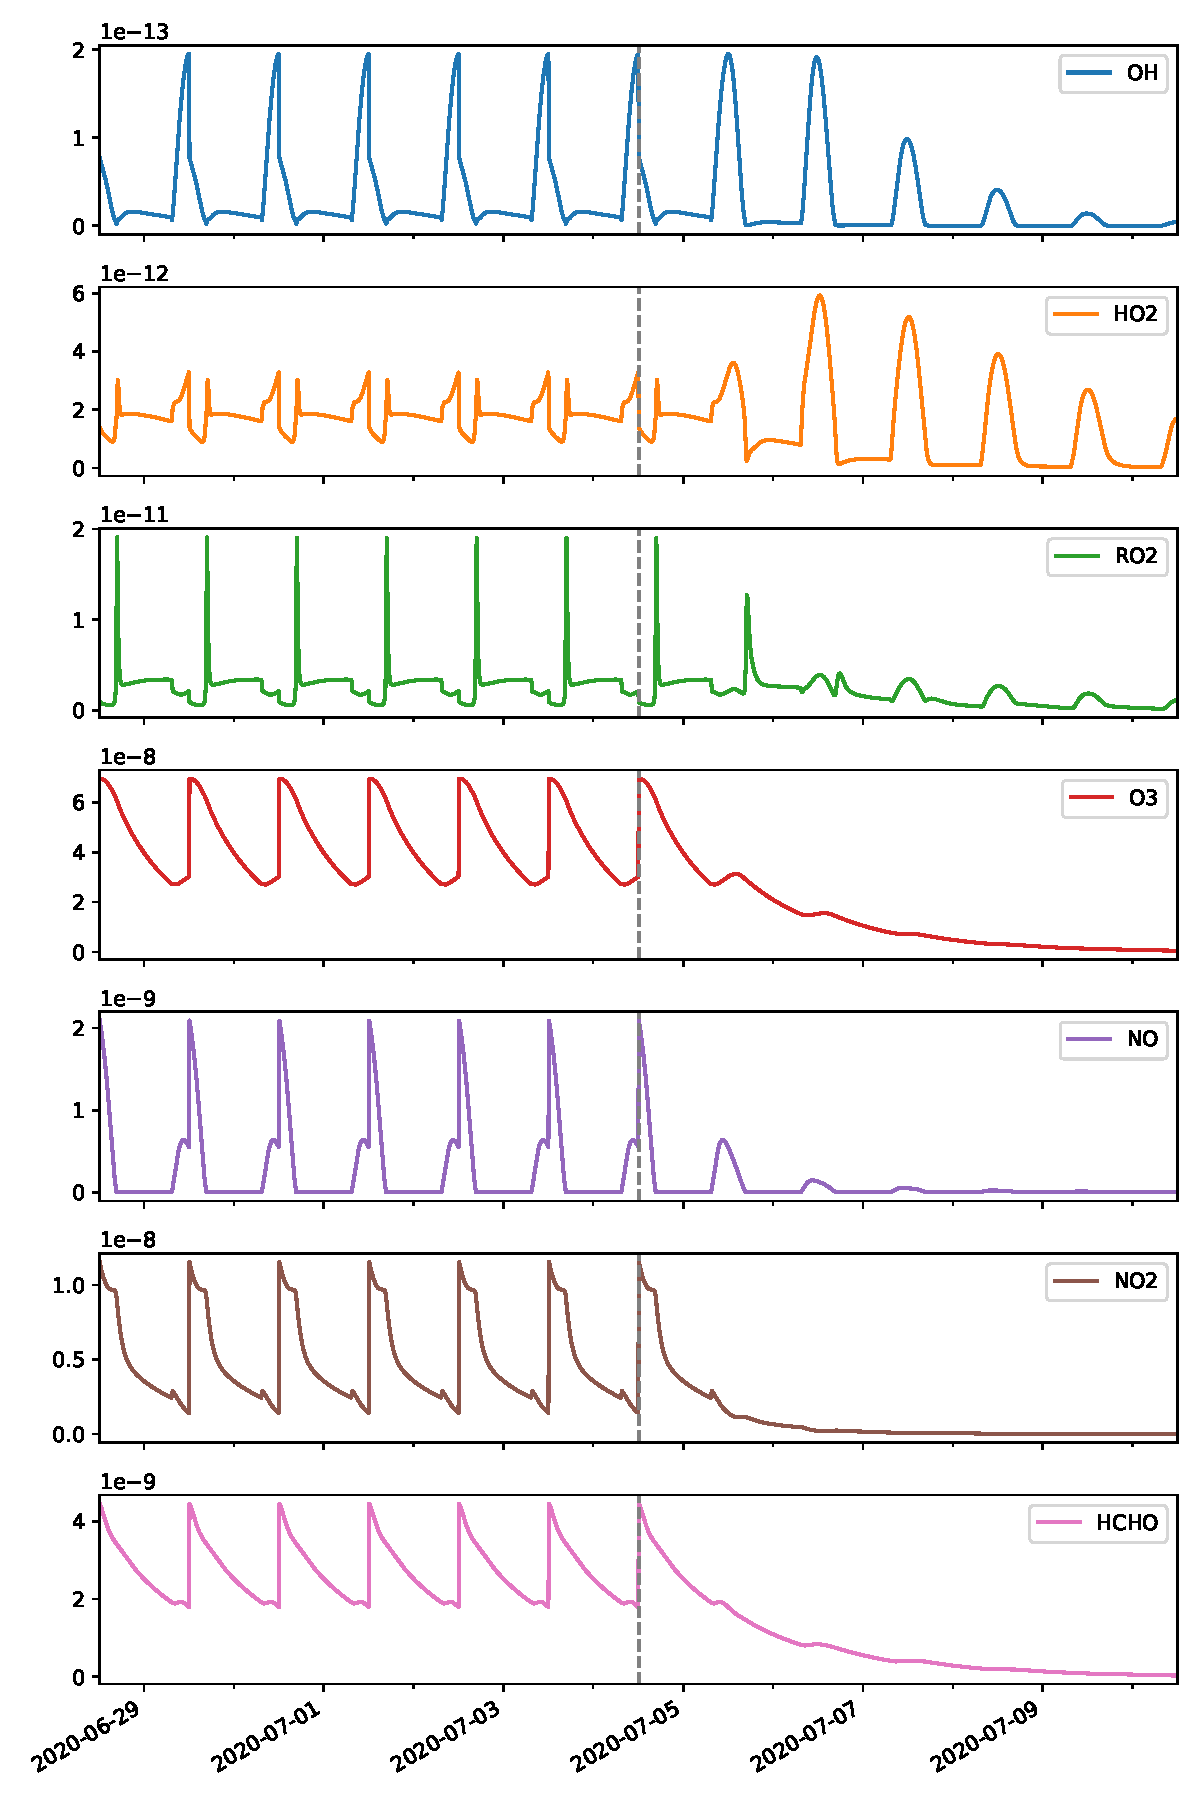
\includegraphics[width=.9\textwidth]{figures_c3/mlpregressor/conc_beijing.pdf}
\caption{\textbf{The concentration profile for Beijing.}This shows a the change in concentration over time for HO$_x$, NO$_x$, Ozone and RO$_2$ species for a simulation run generated by the MLPRegressor. Left of the dashed line shows the last 6 days of spinup, where the initial concentrations are reset at noon each day until the species fractional difference is less than 0.001 .}\label{fig:cbeijing}
\end{figure}

\newpage





\subsubsection{Unifying the results}
Each metric provides a different range in which it ranks the importance of a node. To account for this all results are scaled to the range \{0,1\}, where 1 is the highest. Entries, where the results span several orders of magnitude (e.g. concentration, flux, influence), are flattened using the $\log_{10}$ scale before being normalised. 



\subsection{Comparing Results}
This subsection juxtaposes the use of traditional model diagnostic methods against a selection of graph metrics. As there are several thousand species within each simulation run, the keyword extraction algorithm Term Frequency - Inverse Document Frequency (TF-IDF), is used to identify the top most prominent species for each metric (traditional and graph). From this, the 10 highest-ranking species from each category are collated into a single diagram for comparison. 


\subsubsection{What is TF-IDF}
TF-IDF is a numerical statistic used in text natural language processing and text mining. It is designed to identify the importance of a word concerning its context. 

It provides a value for the frequency a word appears within a document, offset by the number of times it appears in other documents within the corpus - It is for this reason that 83\% of text recommender systems in digital libraries use TF-IDF, \citep{tf83}. 

 In \citep{frankenstein} I applied this to the chapters of Frankenstein and found the keywords extracted almost exactly replicated those from the synoptic description of the novel. Although TF-IDF is a text mining procedure, the algorithm itself is mathematical, meaning that it may be applied to our diagnostic dataset. The working of the algorithm is discussed below.

\paragraph*{Term Frequency}
The TF from the algorithm name stands for term frequency. This is an analysis of the number of times a word exists within a dataset. There are several ways in which this can be done, these are:

\begin{itemize}
    \item[-] \textbf{Raw Count} - The \textit{number of times} a word exists within the document.
    \item[-] \textbf{Boolean/Logistic} - $True$ if the word exists, false otherwise.
    \item[-] \textbf{Adjusted for Document Length} -  $word\ frequency / total\ number\ of\ words$
    \item[-] \textbf{Log Scaled} - $\log(1+frequency)$
\end{itemize}

As the scaled values for each item are taken, we can liken our results to the `Adjusted for Document length' equation and use the scaled ranking value for each group respectively.

\paragraph*{Inverse Document Frequency}
Inverse document frequency tells us how much information a word provides concerning a certain context. Whilst a word may be used extensively throughout the corpus (i.e. term frequency) it is often that we are interested in words which are only frequent within a specific document. This is one of the reasons TF-IDF is useful in the extraction of keywords from a document. 

The inverse frequency of a word is usually calculated as the $\log$ of the fraction of documents $N$ against the number of documents the word appears in $D_f$, \autoref{eqn:idf}.


\begin{equation}
    IDF = \log(\frac{N}{D_f})
    \label{eqn:idf}
\end{equation}

If required, changes can be made to produce results which show a better representation of words which are important for all documents (probabilistic, \autoref{eqn:idfprob}) or individually (smooth, \autoref{eqn:idfsmooth}). However in looking at \autoref{fig:idf}, it can be seen that the basic IDF formula mentioned has a limit of zero the greater the document frequency ($D_f$), which makes it easy to normalise against - i.e. divide by 2 as this is the value tended to if the document frequency tends to 0.    


\begin{equation}
    IDF_{prob} = \log(\frac{N-D_f}{D_f})
    \label{eqn:idfprob}
\end{equation}

\begin{equation}
    IDF_{smooth} = \log(\frac{N}{1+D_f})+1
    \label{eqn:idfsmooth}
\end{equation}




To complete the TF-IDF equation, the term frequency and inverse document frequency terms are multiplied together. 

\paragraph*{Applying TF-IDF to chemical metrics}
To identify metrics selection criteria, we seek only species which are important only in that category. To do this the TF-IDF algorithm can be adapted for use with the graph metric output. Here `Term Frequency' corresponds to the number of times a value appears within the body of a document and can be seen as the scaled \{0,1\} metric output. This is then divided by the log of the `Inverse Document Frequency' with $D_f$ being the sum of values across all the metrics. This makes the TF-IDF equation: 

\begin{equation}
    TF.IDF = metric\_value\  .\ \log(\frac{N_o\ documents}{ \Sigma_\forall\ metric\_values})
\end{equation}


\begin{figure}[H]
     \centering
         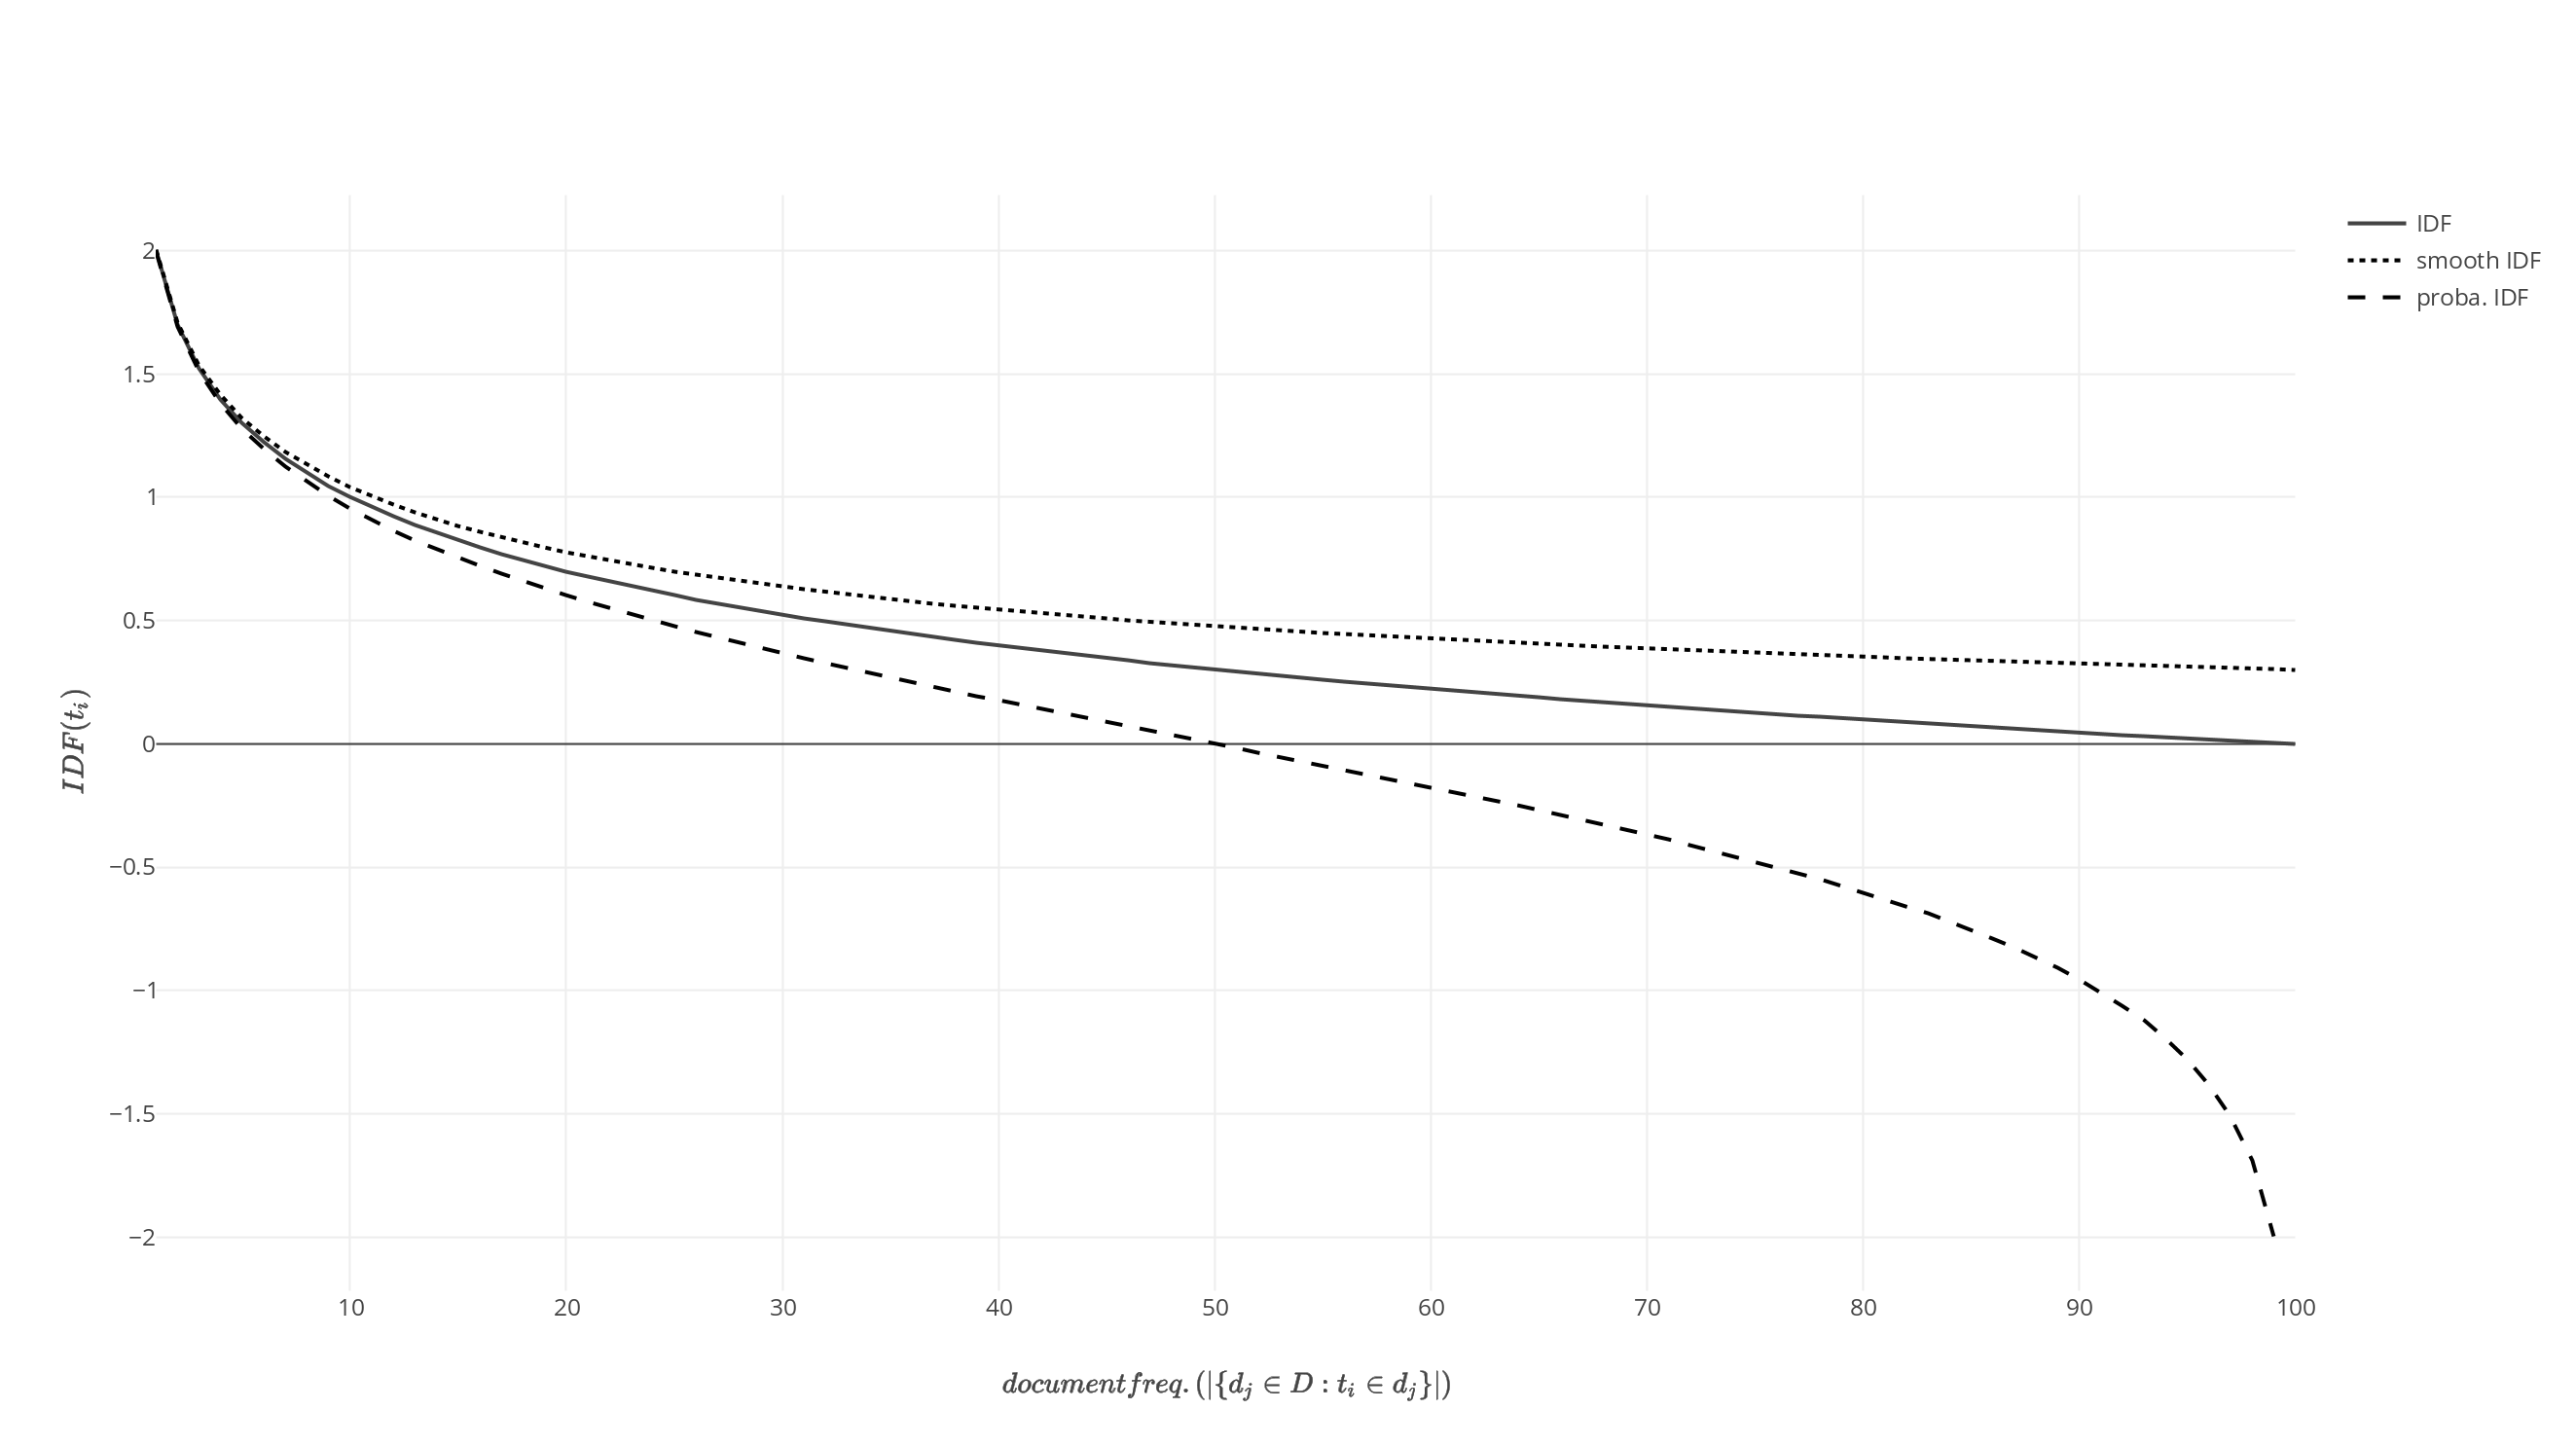
\includegraphics[width=\textwidth]{figures_c3/mlpregressor/plotidf.png}
        \caption{ \textbf{The different IDF outputs.} A plot showing Inverse Document Frequency profiles against Document Frequency. This shows that the probabilistic IDF highlights words that are more important across all items, whilst the smooth IDF shows files which are more important individually. The general IDF (which is used) produces a result starting at 2 and tending to zero. This provides the best response and can easily be scaled between the range of [0,1] by dividing the output by 2.  Source: \citep{idfpic}}
        \label{fig:idf}
\end{figure}




\subsubsection{Metric Comparison}

This section aims to compare the efficiency of graph metrics against a list of traditional methods. To do this the use of a bivariate colourmap (\autoref{fig:cmap}) is used. Each figure consists of a red-hued image/heatmap representing the scaled values \{0,1\}:\{white, red\} for each of the individual columns. As each simulation contains thousands of species, only the top 10 species from each column/category are selected. These are then sorted by the average sum of their closeness, betweenness and page-rank values (blue column). Superimposed on this reds-only heatmap is a blue heatmap representing the average sum of the three metrics for comparison. Such a method allows for the comparison of individual values against an approximation of species importance, by the sum of graph metrics - allowing an easy categorisation of the data:

\begin{itemize}
\item[-] \textbf{Purple} - This value is high in both the individual category and the metric sum. 
\item[-] \textbf{Red} - This value is high for the individual category but not the metric sum. 
\item[-] \textbf{Blue} - This value is high for the metric sum but not the individual category. 
\item[-] \textbf{White} - This value is low for all categories. 
\end{itemize}



\begin{figure}[H]
     \centering
         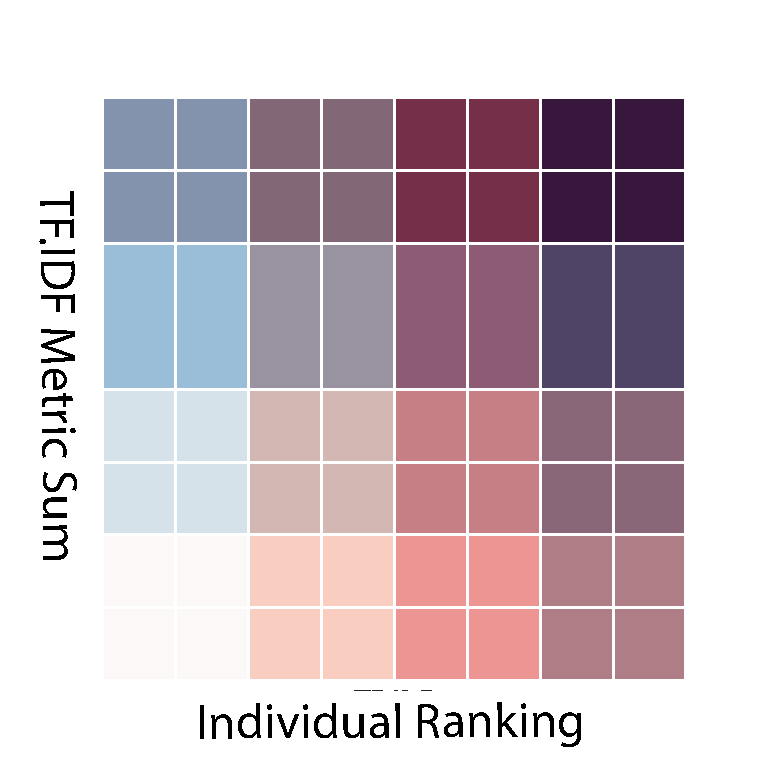
\includegraphics[width=0.4\textwidth,angle=45]{figures_c3/mlpregressor/cbar.pdf}
        \caption{ \textbf{The bivariate colourplot key.} }
        \label{fig:cmap}
\end{figure}


\subsubsection{Individual Categories}
Individual categories are split between traditional metrics and graph centrality metrics. To represent the importance of a species the following values may be extracted through the use of a simple box model:

\begin{itemize}
\item[-] \textbf{Concentration} - This describes the abundance of a species within the atmosphere. 
\item[-] \textbf{Net Flux} - This describes the rate of net (absolute) change of concentration over time for a species. 
\item[-] \textbf{Absolute Flux} - Some species may have a large flux going through them (production and loss), resulting in a small net flux. This sums the production and loss fluxes. 
\item[-] \textbf{Influence} - Influence is the total magnitude of an effect that changing a species concentration by 1\% would have on other species within the network. Since the graph is generated using the Jacobian matrix, an alternative method for calculating this can be by calculating the total out-degree of a node.  
\end{itemize}



The importance of a species is then compared through the use of three of the most common centrality metrics. These are:


\begin{itemize}
\item[-] \textbf{Centrality} - This describes how easily information from one node can be disseminated to all other nodes. 
\item[-] \textbf{Betweenness} - This describes the number of shortest paths (fastest fluxes/greatest influences) that are routed between nodes adjacent to our chosen node. Species with a high betweenness hold a brokering position and can act as a bottleneck between different groups of chemistry. 
\item[-] \textbf{PageRank} - PageRank looks at the flow in a system. It ranks nodes not only on the number of species it reacts with but also the importance of the species it has reacted with.

\end{itemize}

Finally, the `Metric Sum' is the sum of all the metric values scaled between 1 and zero (the mean).

\subsection{Senario Analysis}
In selecting the top 10 ranking species for each category it is possible to examine if the importance of a species with centrality metrics varies from the results suggested by traditional metrics. In this subsection, we explore the TF-IDF rankings of each metric and use this to decide if species importance is local to a specific metric. We look at what species are highlighted by each scenario and compare them against the primary emitted species shown in \autoref{tab:icsmetric}. Finally, we compare the total metric sum against the traditional metrics of concentration and flux and compare the correlation. 

\subsection*{Cape Verde}
The initial conditions for Cape Verde have low levels of NO$_x$ and ozone. The chemistry is split between aromatics and small alkanes. The aromatic species are of a similar magnitude to the alkanes. Many of the aromatic products are shown to be important in \autoref{fig:heatcv}, which may be due to the larger aromatic species <break down?> potential (they have more carbons to form bonds with). Using this it can be seen that many of the species highlighted are products of Toluene, Benzene, Phenol and Catechol (the latter of which are produced by adding an alcohol group to a Benzene ring - \autoref{fig:aromaticbz}). These are most likely emitted either from mainland Africa or through ship emissions and are important indicators of how processed the chemistry of the atmosphere is. Benzene and Toluene are usually emitted at a ratio of 1:4 respectively and the same rate. Since Toluene reacts at a much faster rate, a change to this ratio allows tells us how much the chemistry within a system has changed. It may be suggested both from the initial conditions and the metrics that the chemistry is one which has been transported to the island, rather than emitted there. In addition to the aromatics, many of the primary emitted alkanes, and their products, have been highlighted. These tend to be unreactive (and thus long-lived) which can be seen by their low betweenness\footnote{Most of the species with low betweenness values are a product of Ethane (\ch{c2h6}), Propane (\ch{c3h8}), Butane (\ch{c4h8}) and Pentane (\ch{c5h12})} values - they are unlikely to act as a fast-reacting proxy between two other species. The change in colour between the metrics suggests that for the Cape Verde Mechanism important species are not often central (easy to get to - closeness centrality) from all other species. The selected species ranking the highest closeness (Propane-Pentane) do not seem to be ranked important as part of betweenness or page rank which results in the red colour for the plot (low overall metric sum). Species ranked high by the PageRank algorithm do not have a high betweenness or net flux value, but do have large absolute flux. This suggests that although they may not have the fastest fluxes going through them (low betweenness), they act as an intermediate reaction for other chemistry where they are produced and lost at a similar rate (low net flux, high absolute flux. ). 


\begin{figure}[H]
    \centering
\begin{subfigure}[b]{.14\textwidth}
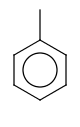
\includegraphics[width=\textwidth]{figures_c3/TOLUENE.png}
\caption{Toluene}
\end{subfigure}
\begin{subfigure}[b]{.14\textwidth}

\includegraphics[width=\textwidth]{figures_c3/BENZENE.png}
\caption{Benzene}
\end{subfigure}
\begin{subfigure}[b]{.14\textwidth}
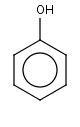
\includegraphics[width=\textwidth]{figures_c3/PHENOL.png}
\caption{Phenol}
\end{subfigure}
\begin{subfigure}[b]{.19\textwidth}
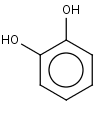
\includegraphics[width=\textwidth]{figures_c3/CATECHOL.png}
\caption{Catechol}
\end{subfigure}
\caption{\textbf{Chemical structures of the 4 most common type of aromatic species in cape verde.}}
\label{fig:aromaticbz}
\end{figure}

  
\subsection*{Borneo}
The Borneo dataset, through the nature of being located in a rainforest, contains no benzene ring based aromatics. From its initial conditions the simulation begins with a higher level of Ozone, High Isoprene (\ch{c5h8}), and moderate amounts of Acetylene (\ch{c2h2}), $\alpha$-pinene, and limonene (both (\ch{C10H16})). \autoref{fig:heatb} shows a very large of the rainforest chemistry is dominated by terpenes (mainly Isoprene) products. Unlike Cape Verde, these all have a high concentration, net-flux and absolute flux. This suggests that the products act as intermediate species for the chemistry and are both produced and lost at a high rate. Much of these species have a high closeness and a high page rank, suggesting that the centre of the Borneo network is very close-knit, and the well connected to species of importance. The only outlier to this is \ch{cisopao2} which is has fast reactions flowing through it and has important connections (it is only a couple of steps away from Isoprene) but does not have a high closeness centrality. This suggests that it is located as part of a terpene branch but not at a highly pivotal position. The uniformly distributed colour gradient for betweenness suggests that there are many possible reaction routes a species may undergo before being converted into carbon dioxide and water. The exception to this is \ch{c517chO} which has 14 precursors and only 2 products (a bottleneck / pivotal position), resulting in the highest betweenness value of the network. 


\subsection*{London}
The London dataset contains a mix of anthropogenic and biogenic aromatics and long-chain alkanes. Similar to Cape Verde we have a section of alkanes which have a low overall metric sum, with a small value for closeness and page rank. Combined with their high net flux, absolute flux and influence values, this suggests that they have a moderate directional flux, most likely influencing the production of many other species at a consistent rate. In addition to these, we have species with a moderate closeness but a high betweenness. These are often species such as formaldehyde (\ch{HCHO}), glyoxal (\ch{c2o2}) and acetaldehyde (\ch{ch3co3}) which can serve as tracers for fast photolytic reactions. This is because on the graph structure (\autoref{MCM ALL or VanKrevlin graph}) they sit between the dense centre of the network (high closeness) and the branches formed from each primary emitted species (low closeness). Their high connection density and importance in the network is also picked up by the page rank algorithm. Other species with high betweenness and a low centrality are the monoterpenes limonene and $\alpha$ pinene, as well as hexane (\ch{nc6h14}) and butane products. These are (or are close to) primary emitted species and therefore have a low closeness. Since this also means that much of the chemistry originates with them, the outward 'flow' of information also results in a lower page rank value. 

\subsection*{Beijing}
Similar to London, the fast photochemical tracers are identified, although some have a slightly lower flux between them (betweenness) and page rank values. This suggests that the network structure or weightings may have shifted slightly, creating more links, or importance in a specific branch of chemistry. 
 Additionally, their overall metric sum is lower. Glyoxal, Methyl Vinyl Ketone (MVK) and their associated criegee configurations all feature heavily in the middle of \autoref{fig:heatbj}. These are important as they represent the fast chemistry formed by both the anthropogenic and biogenic chemistry that is within the simulation. These tend to have a high closeness and page rank centrality, a pattern that is also seen with the long-chain alkane products from Octane (\ch{NC8H18}), Hexane (\ch{nc6h14}) and isoprene.



\begin{figure}[H]
     \centering
         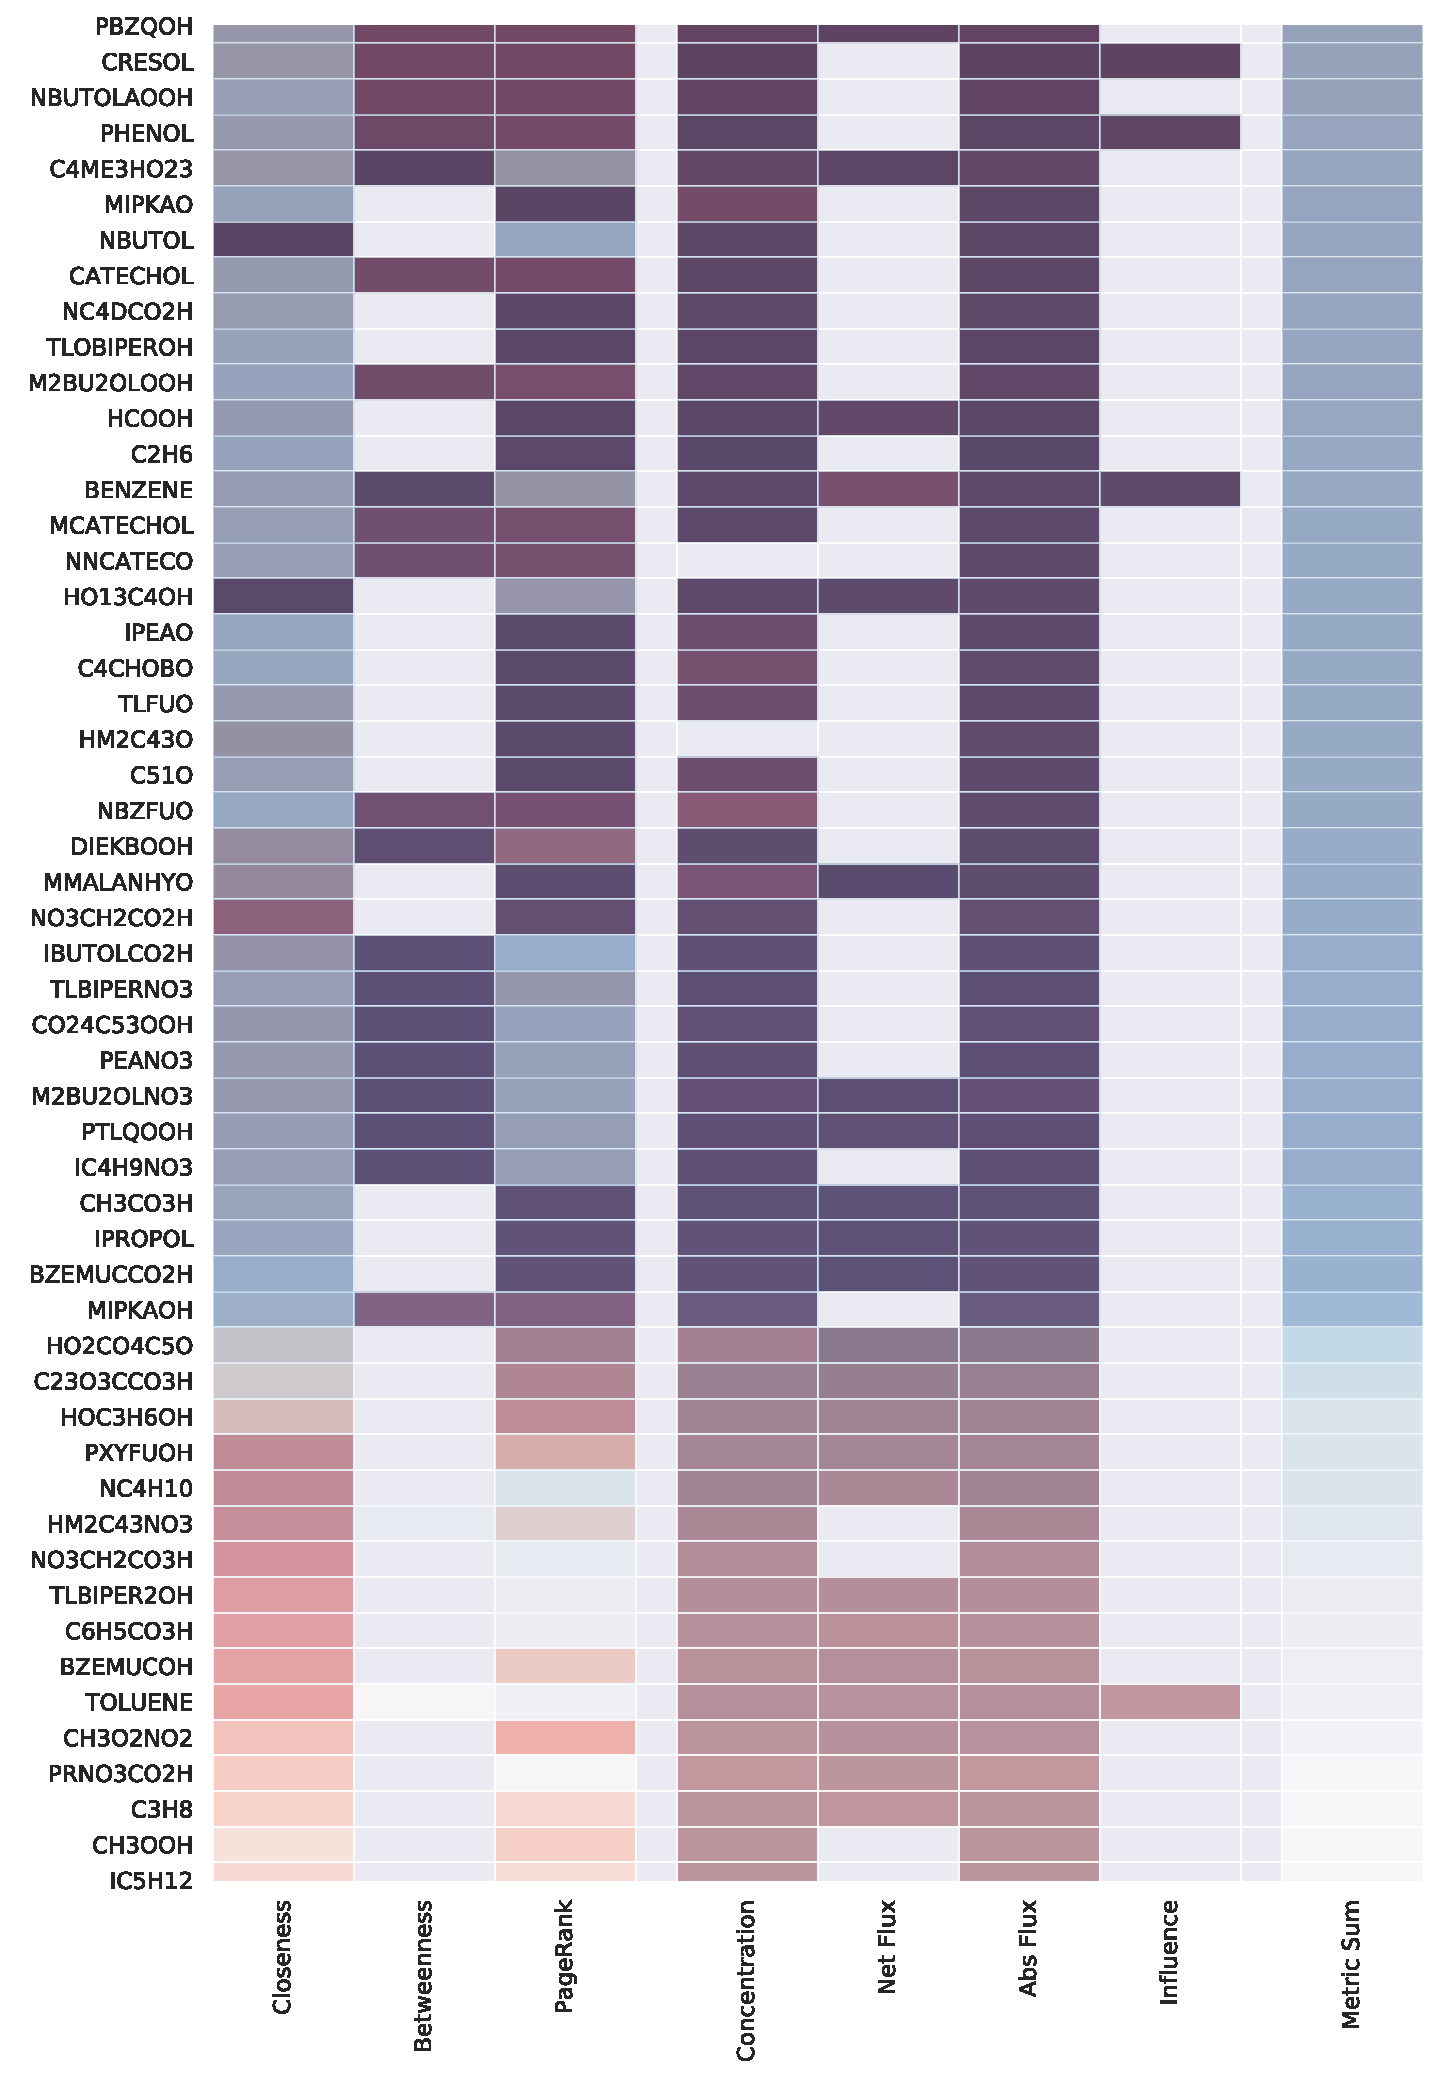
\includegraphics[width=.95\textwidth]{figures_c3/mlpregressor/cape_CapeVerde.pdf}
        \caption{ \textbf{A bivariate heatmap comparison of Cape Verde.} }
        \label{fig:heatcv}
\end{figure}

\begin{figure}[H]
     \centering
         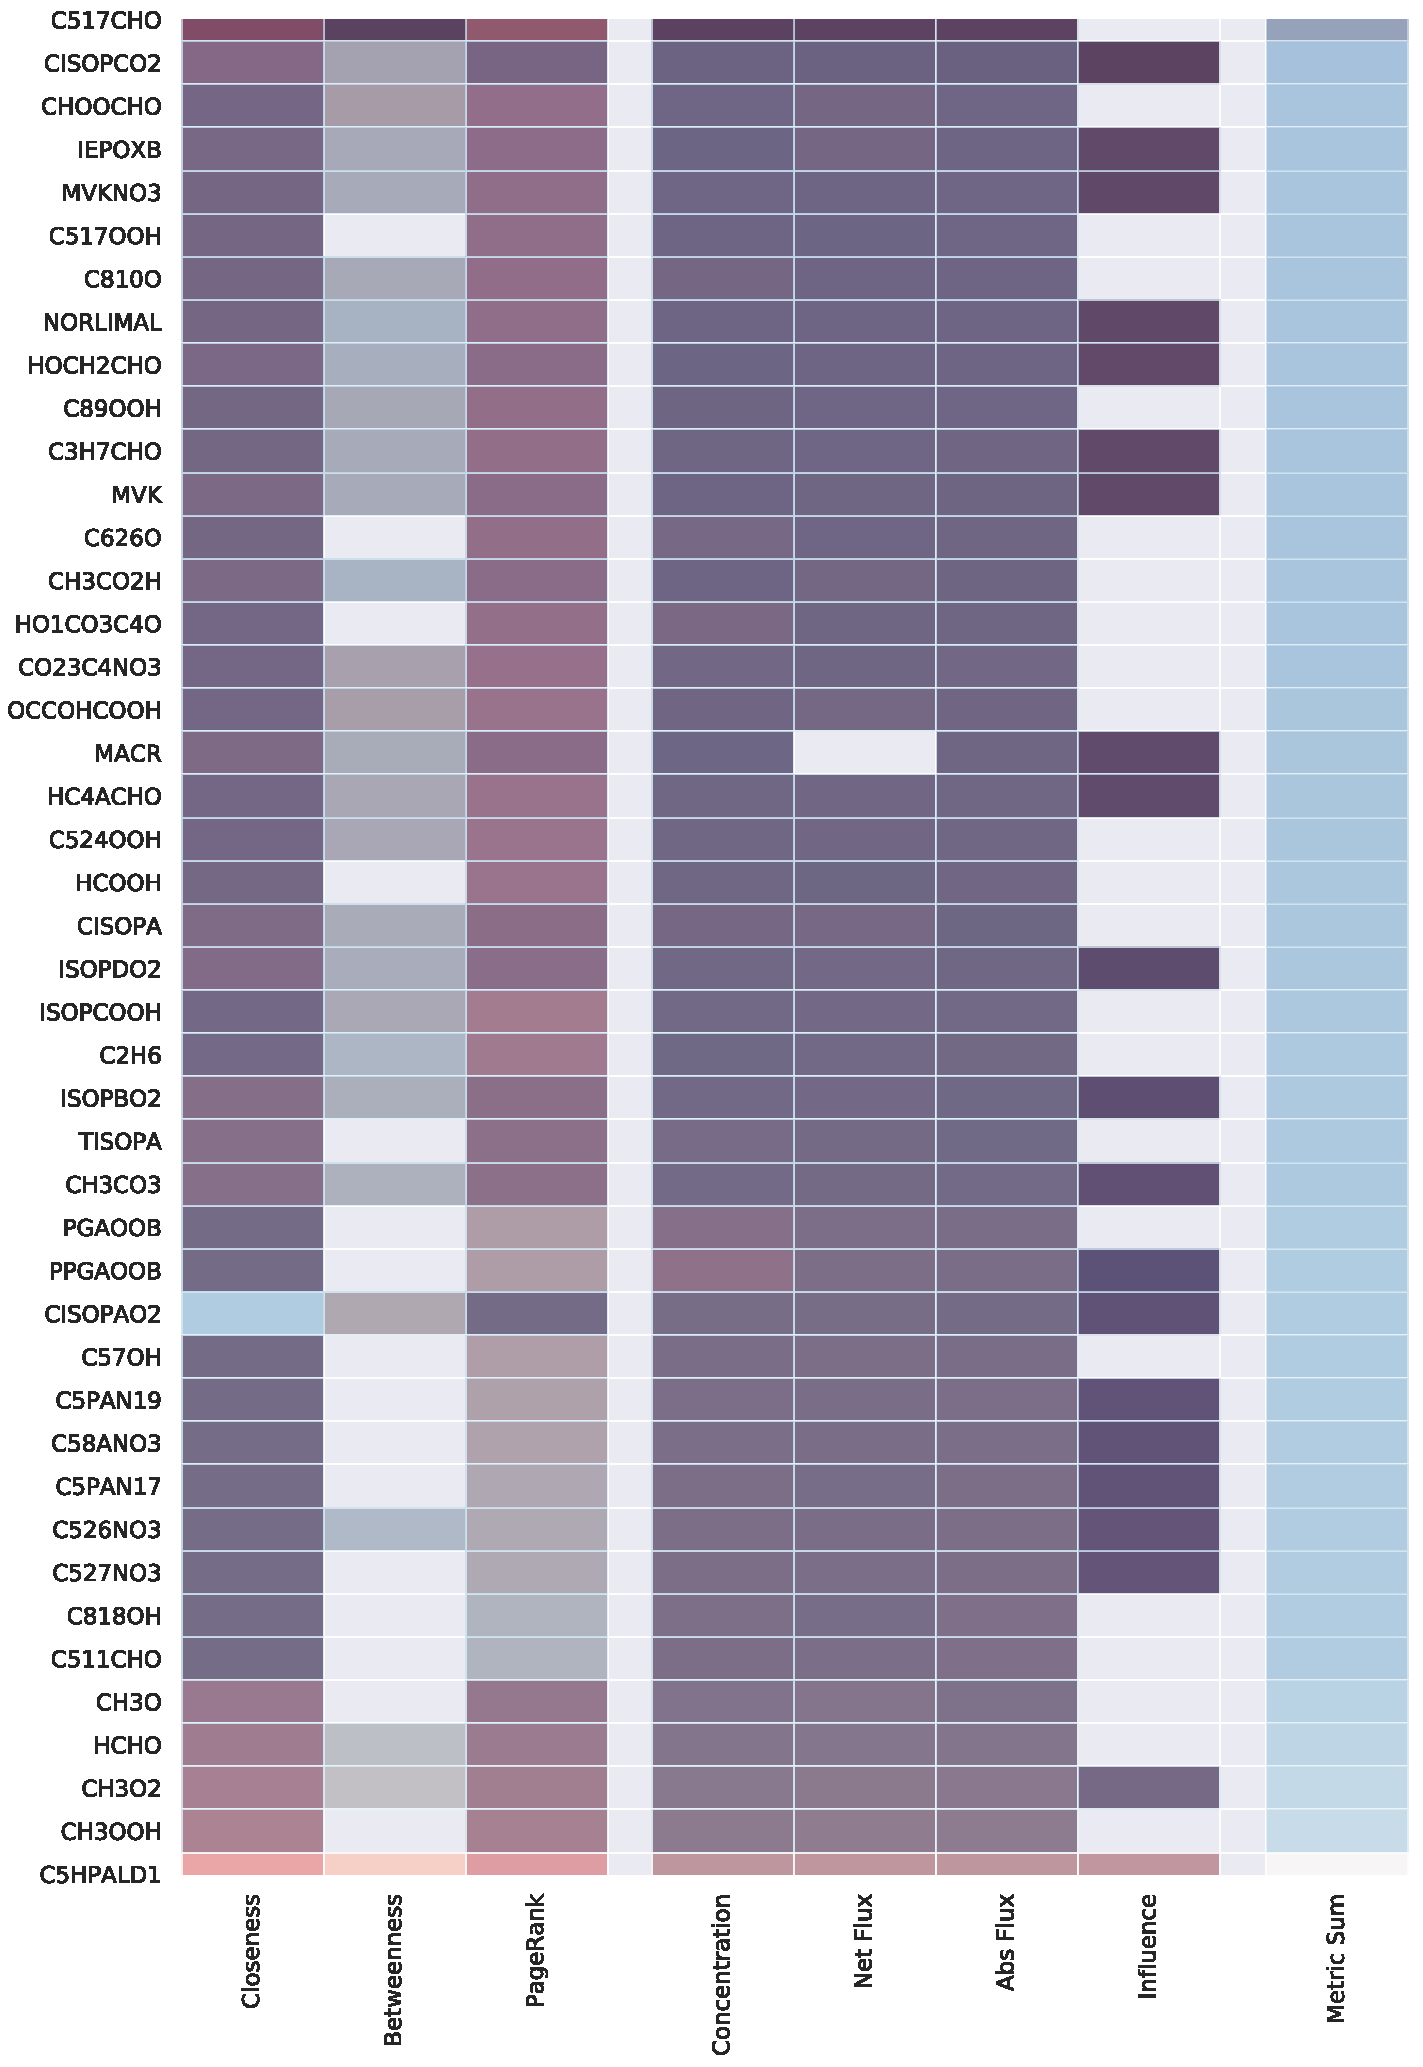
\includegraphics[width=.95\textwidth]{figures_c3/mlpregressor/op3_Borneo.pdf}
        \caption{ \textbf{A bivariate heatmap comparison of Borneo.} }
        \label{fig:heatb}
\end{figure}

\begin{figure}[H]
     \centering
         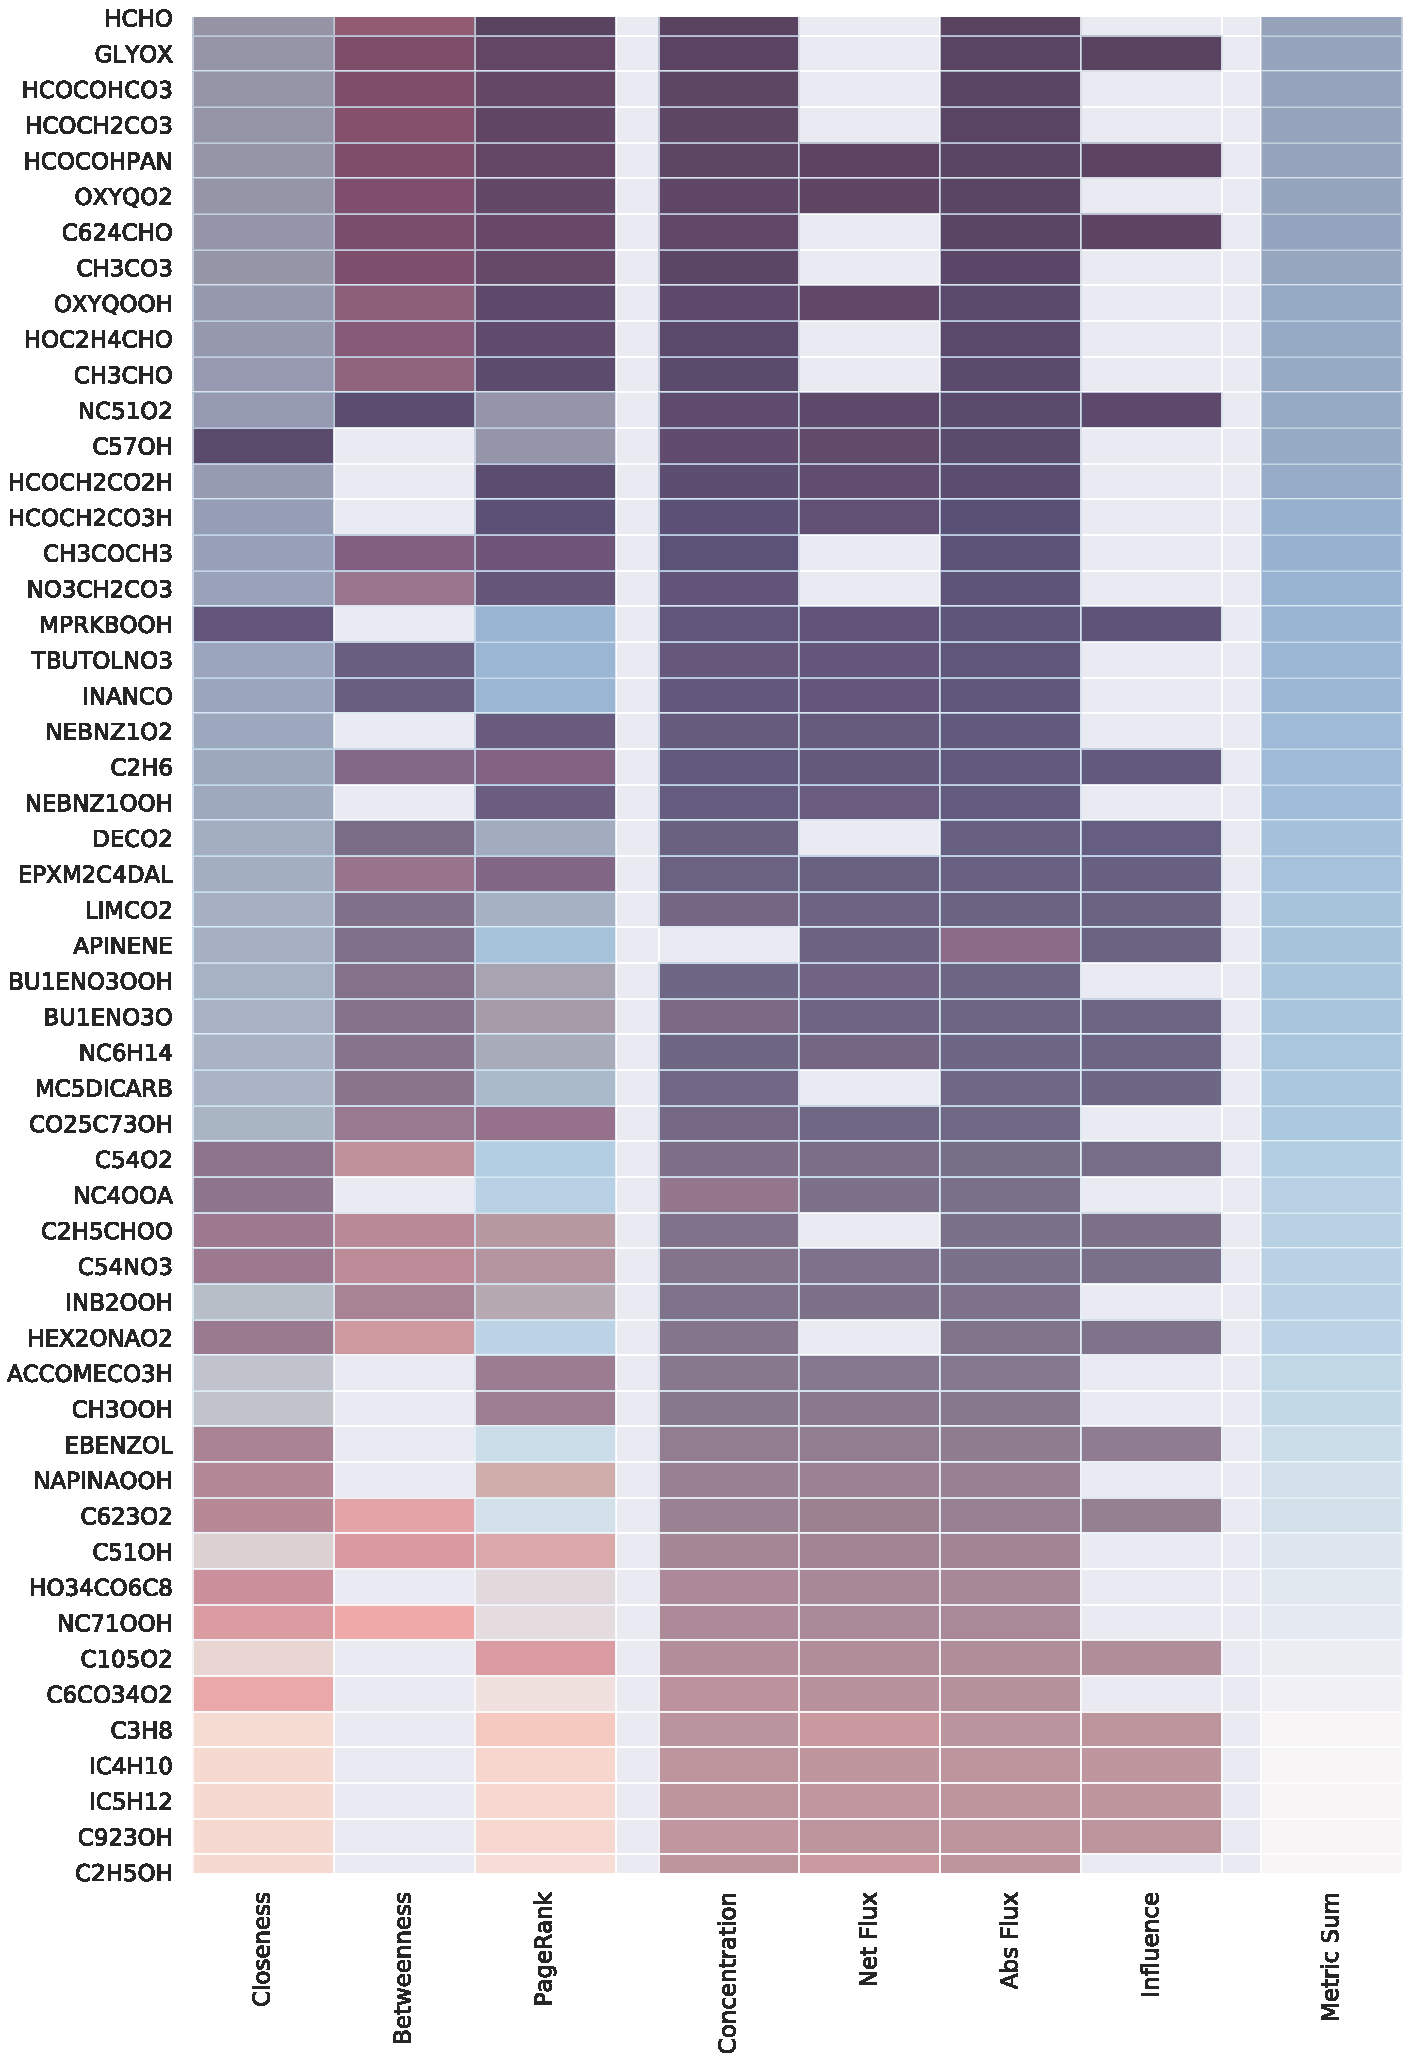
\includegraphics[width=.95\textwidth]{figures_c3/mlpregressor/clfo_London.pdf}
        \caption{ \textbf{A bivariate heatmap comparison of London.} }
        \label{fig:heatl}
\end{figure}

\begin{figure}[H]
     \centering
         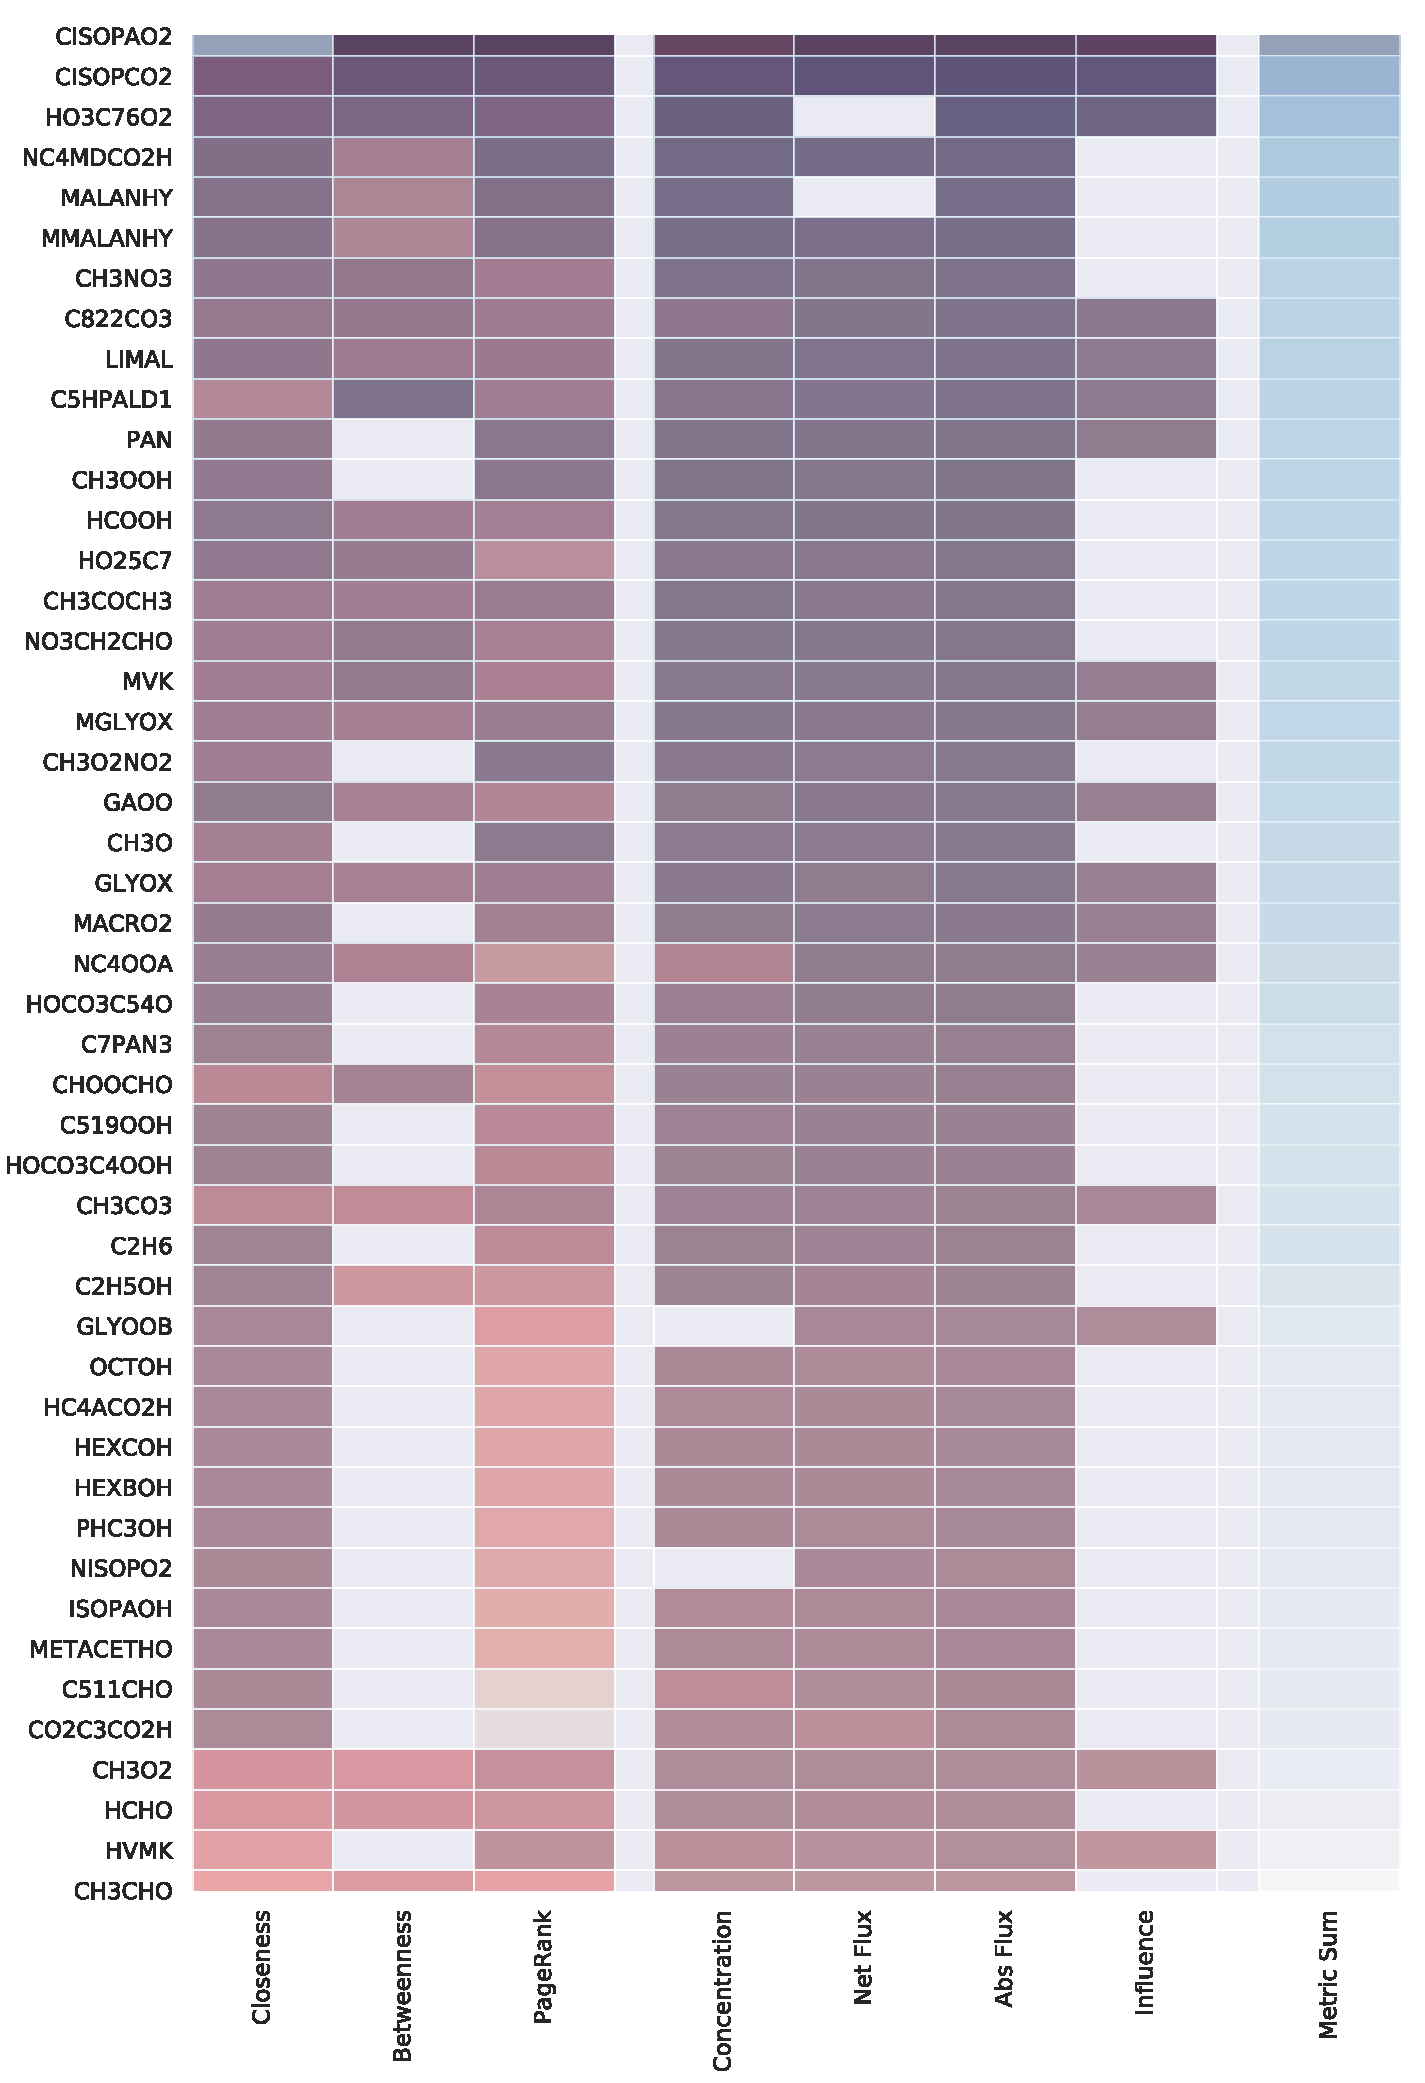
\includegraphics[width=.95\textwidth]{figures_c3/mlpregressor/aphh_Beijing.pdf}
        \caption{ \textbf{A bivariate heatmap comparison of Beijing.} }
        \label{fig:heatbj}
\end{figure}




  
\subsubsection*{Ability to match traditional metrics}
All graph construction
Colours - all purple, suggests a general agreement
photochemical tracers

\subsection{Providing an overall overview using the TF-IDF and the metric sum.}
In the previous section, it was shown that centrality metrics can be used to complement the use of traditional metrics in the analysis of the chemical network. As each metric represents a different aspect of importance, should a single ranking value for a node be required, it is possible to take the average sum of all three metric values. Looking at \multiref{fig:heatcv}{fig:heatbj} it is possible to see similar trends in colour gradient between the purples of the traditional metrics of flux and concentration with the total metric sum (the blue column). This suggests that it is possible to compare each scenario with the use of the metric sum. 

In selecting the ten highest-ranking species from the mean centrality metric table for each simulation, \autoref{tab:groupcomp} can be created. Unlike the previous method, we are now looking at species which are important across all metrics in a simulation. For Borneo species produced from Heptane, Hexane, Isoprene and Limonene are seen as important. Cape Verde, similar to before, has a selection of Benzine related products such as Phenolic and Catecholic compounds. Beijing consists mainly of Quinones and Dialdehydes which are both derivatives of Benzene. London again has Benzine related compounds, mixed with the fast photochemical indicators, which were also ranked highly in \autoref{fig:heatl}. Looking at the highest-ranking sum (Nan-mean), it is seen that isoprene, hept/hexane and glyoxal products highlighted as the most consistently important across all four simulations. 

\begin{table}[H]
\centering
\small
\begin{tabular}{llllll}
\toprule
{} &         London &         Cape Verde &           Beijing &           Borneo &          Nan-Mean \\
\midrule
0 &       \ {HCHO} &      \ {PBZQOH} &     \ {PTLQONE} &     \ {C622OH} &    \ {CISOPCO2} \\
1 &     \ {CH3CHO} &      \ {PHENOL} &     \ {PBZQONE} &     \ {C923OH} &    \ {CISOPAO2} \\
2 &  \ {C5CO14OOH} &  \ {C24O3CCO2H} &  \ {HOHOC4DIAL} &      \ {C54OH} &     \ {C517CHO} \\
3 &    \ {PBZQOOH} &    \ {NBZFUONE} &  \ {MNNCATCOOH} &    \ {HO2C4OH} &     \ {HO2C6O2} \\
4 &    \ {MALANHY} &  \ {TLBIPERNO3} &    \ {C6H5CO3H} &     \ {C624OH} &   \ {HCOCH2CO3} \\
5 &     \ {CH3CO3} &    \ {BZBIPERO} &    \ {EPXDLPAN} &     \ {HEXAOH} &      \ {C717O2} \\
6 &      \ {C57OH} &  \ {TLEMUCCO2H} &     \ {C5DIALO} &   \ {C822CO2H} &   \ {HCOCOHCO3} \\
7 &    \ {C624CHO} &  \ {BZEMUCCO2H} &    \ {NBZFUOOH} &  \ {MACROHOOH} &  \ {HOCH2CH2O2} \\
8 &      \ {GLYOX} &       \ {PTLQO} &  \ {TLBIPEROOH} &  \ {HO14CO2C4} &   \ {HOC2H4CHO} \\
9 &  \ {HCOCOHCO3} &    \ {NNCATECO} &    \ {NCRESOOH} &   \ {C624CO2H} &     \ {C626CHO} \\
\bottomrule
\end{tabular}
\caption{\textbf{A table of the top 10 ranked species for each simulation.} Only species that exist within atleast 3 out of the 4 simulation are used. The Nan-Mean takes the mean of all available data, ignoring runs where a species is not present.}
\label{tab:groupcomp}
\end{table} 



\textit{\textbf{A note on finding the precursors}\\ Graphs are also useful in the back navigation of a network. It is possible to discover the most probable primary emitted species (nodes with no in-degree) by comparing the shortest path lengths for all primary emitted species (not including inorganic species). Here the primary emitted species with the smallest number of connections are often the most likely source.}




\section{Calculating production sensitivity using personalised page rank.}

In \label{sec:pagerank} the calculation of the PageRank result by solving for the eigenvalues and vectors of the google matrix was discussed. It was also mentioned that an equivalent method to get a result may be obtained by propagating the one's vector in small increments, \autoref{eqn:forwards}. This works much like the integrator within a chemical box model, except rather than updating the species concentration with each time step, we move information between each node. 

Using this analogy it, therefore, follows that should we reverse the direction of the flow (change the edges from source $\rightarrow$ target to source $\leftarrow$) it would be possible to see where species influence originates, \autoref{fig:prgraphs}. As each network is constructed directly from the Jacobian matrix (what is used within the integrator to propagate a model forwards in time ), reversing the link direction is analogous to taking the transpose of the jacobian. Within the modelling world, the resultant matrix is now known as the adjoint. The adjoint matrix is often used in the running of models backwards in time, to make historic predictions based on current data. 

\textbf{Some information on using the adjoint and references here }



% http://sibiu.cs.vt.edu/eprints/id/eprint/282/1/Sandu_2003_KPPSEN1.pdf
% The adjoint modelling is presented as an eclient tool to evaluate the sensitivity
% of a scalar response function with respect to the initial conditions and model parameters. In addition,
% sensitivity with respect to time dependent model parameters may be obtained through a single backward
% integration of the adjoint model

\begin{figure}[H]
    \centering
\begin{subfigure}{.9\textwidth}
  \centering
  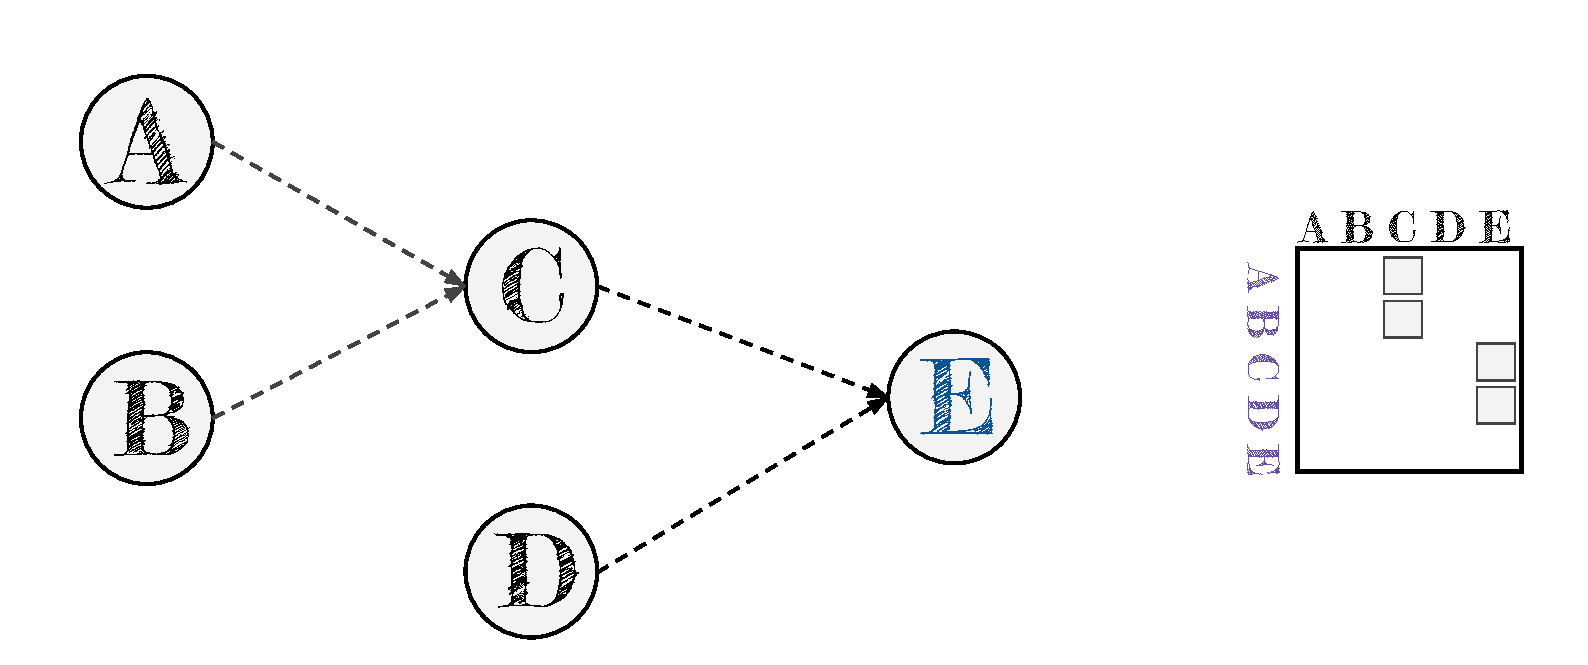
\includegraphics[width=\textwidth]{figures_c3/traditional.pdf}
  \caption{Traditional Influence Graph} 
\end{subfigure}

\begin{subfigure}{.9\textwidth }
  \centering
  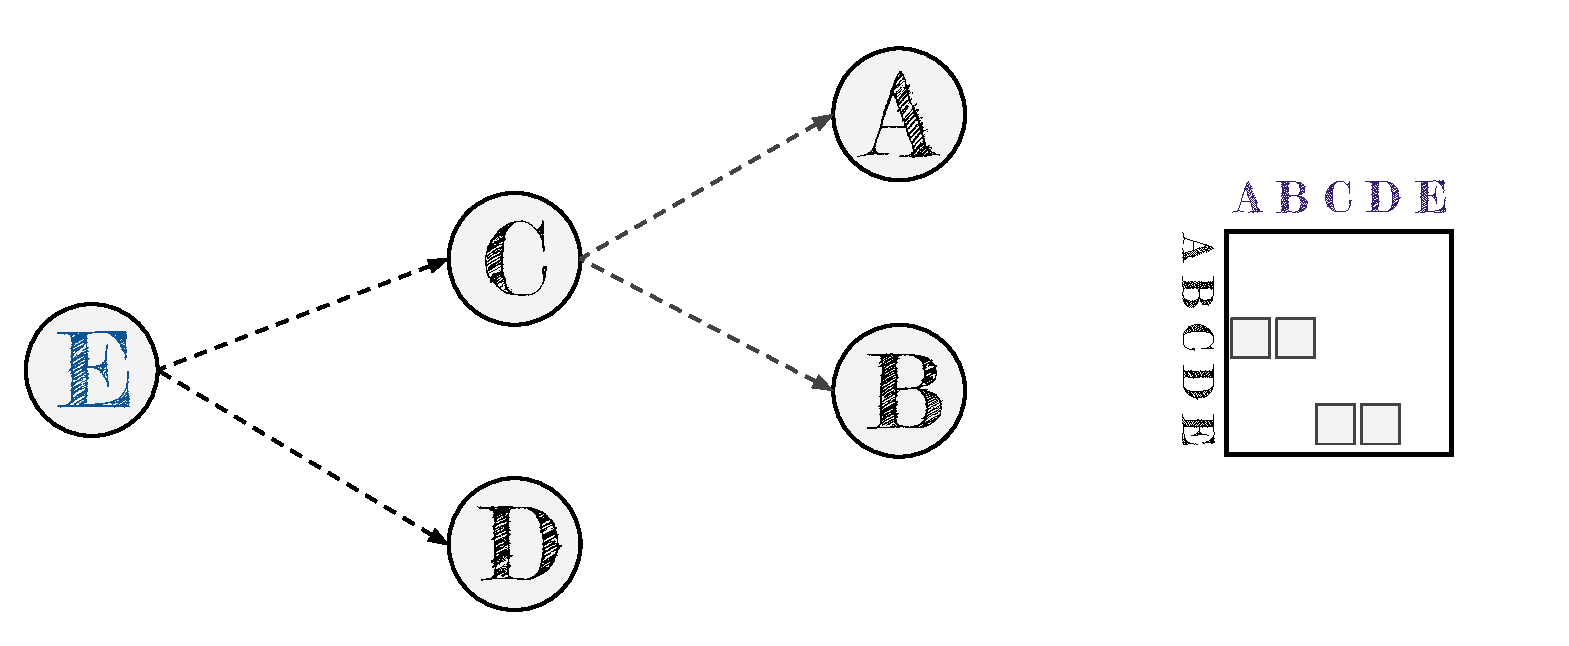
\includegraphics[width=\textwidth]{figures_c3/adjoint.pdf}
  \caption{Reversed-link (adjoint) influence graph}
\end{subfigure}

\caption{\textbf{Link reversal of the Jacobian Sensitivity matrix graph results in a graph of the Adjoint.} Showing how in changing the direction of the links in a graph is equivalent to applying the transpose to an adjacency matrix (right). In the case of a Jacobian based graph, this is analogous to using the adjoint to propagate the model back in time - something that can be used to identify the influence upon a species with a model.}
  \label{fig:prgraphs}
\end{figure}




\subsection{Testing}
As with all scientific processes, it is important to first test the algorithm on a small, comprehensible example. To do this we start with the creation of \ch{ch2oo} within the Borneo mechanism. This is a direct product of isoprene. In tracing back all the species precursors the mechanism for its creation can be described as: 

\begin{equation}
    \ce{O3 + C5H8 ->[\kappa] CH2OOE}+(MACR\ or\ MVK)
\end{equation}
\begin{equation}
    \ce{CH2OOE ->[\kappa_{dec}] CH2OO}
\end{equation}
In traversing the adjoint/reversed graph, this presents a singe `shortest path' between the product and its precursor. This creates a base test for the algorithm. The PageRank algorithm is now run with a personalisation vector consisting of a value of 1000000 for the species of interest and -1 for all others. A damping factor value of 0.01 is also used for the algorithm. 

As \ce{CH2OOE} only has one precursor ($\alpha$-pinene) the initial test is done on this. From this, the identification of isoprene as a source is successful, although since the algorithm is performed on the whole network, there are results for several additional species, \autoref{tab:ch2ooe}. This is because page rank works on using teleportation to change between items in the evolution of the system. With the design of the personalisation vector, these values will, however, be significantly smaller than any containing useful results. 


\begin{table}[H]
    \centering
    
    \begin{tabular}{lr}
\toprule
\ch{C5H8}    &  9.920000e-03 \\
\ch{CH2OOE}  &  9.920000e-01 \\
\midrule
\ch{C816O}   & -9.990000e-07 \\
\ch{NC101CO} & -9.990000e-07 \\
\ch{C926OH}  & -9.990000e-07 \\
\bottomrule
\end{tabular}
\caption{A reversed graph Page Rank test with \ce{C5H8 + O3 -> CH2OOE} as the only reaction.}
\label{tab:ch2ooe}
\end{table} 

Next, we apply the same methodology to \ce{CH2OO}. This creates the graph in \autoref{fig:prtest0}. Here it is seen that \ce{CH2OO} is directly dependant on the radicals \ce{CH2OO[F,B,C,G,A]}, and \ce{CH2OOE}. This is then dependant on Isoprene, which then has a range of dependencies with all have precursors of their own (not shown). \autoref{tab:ch2oo} shows the direct dependence on Isoprene and the criegee radicals of \ch{ch2oo} in addition to  


\begin{figure}[H]
  \centering
  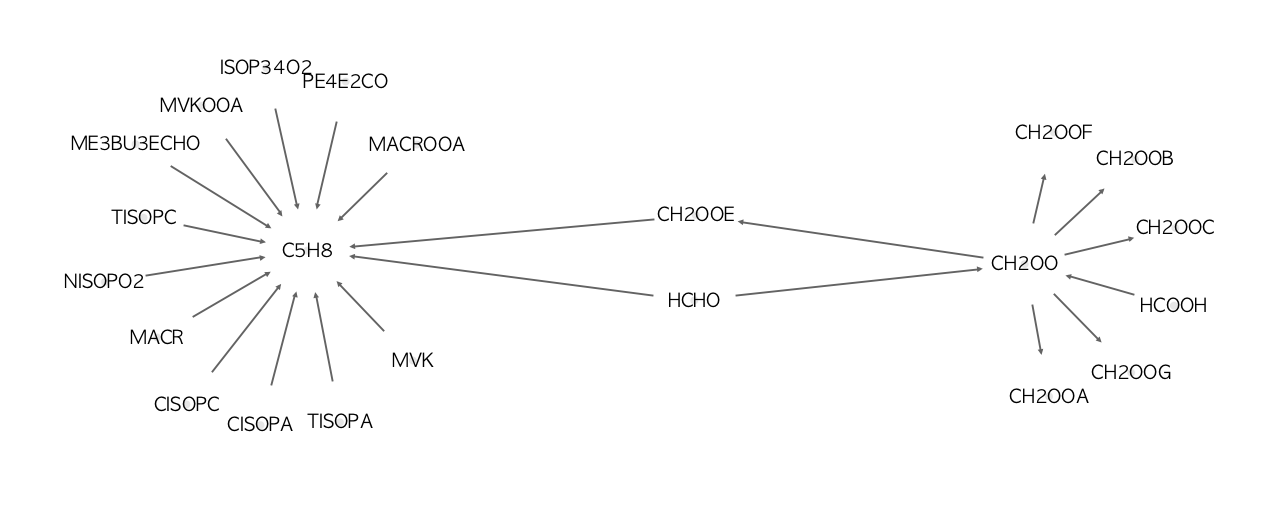
\includegraphics[width=\textwidth]{figures_c3/prtest0.png}
\caption{\textbf{The reversed subgraph between Isoprene, \ce{CH2OOE} and \ce{CH2OO}.} This is a subgraph of the afforementioned species, showing them and their neighbours. Here the arrows point towards a species precursor. }
\label{fig:prtest0}
\end{figure}

\begin{table}[H]
    \centering
    \begin{tabular}[width=\textwidth]{lr}
    \toprule
    CH2OO      &  0.992000 \\
    CH2OOE     &  0.001670 \\
    CH2OOF     &  0.001660 \\
    CH2OOG     &  0.001660 \\
    CH2OOA     &  0.001660 \\
    CH2OOC     &  0.001640 \\
    CH2OOB     &  0.001640 \\
    C5H8       &  0.000016 \\
    \midrule
    MACR       &  0.000016 \\
    C2H4       &  0.000007 \\
    HMACR      &  0.000007 \\
    ISOP34NO3  &  0.000005 \\
    \bottomrule
    \end{tabular}
\caption{A reversed graph Page Rank test with \ce{CH2OOE}, small constent values have been removed.}
\label{tab:ch2oo}
\end{table} 

Next, a test using $\alpha$ pinene with a bit more chemistry is done. 


\begin{figure}[H]
  \centering
  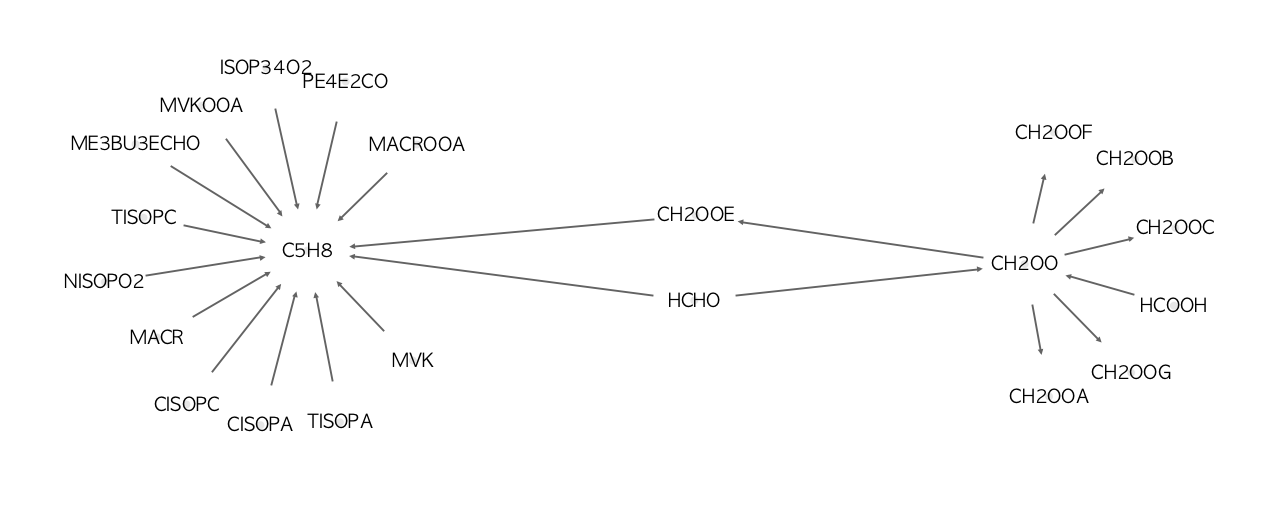
\includegraphics[width=\textwidth]{figures_c3/prtest0.png}
\caption{\textbf{The reversed subgraph between $\alpha$-pinene, and \ce{NC101CO}} This is a subgraph of the afforementioned species, showing them and their neighbours. Here the arrows point towards a species precursor. }
\label{fig:prtest1}
\end{figure}


\begin{table}[H]
\centering
\begin{tabular}{p{.4\textwidth}p{.4\textwidth}}
\toprule
NC101CO   &  9.920000e-01 \\
APINENE   &  9.210000e-06 \\
NAPINBO   &  4.540000e-03 \\
NAPINBO2  &  2.770000e-03 \\
NAPINBOOH &  2.690000e-03 \\
\midrule
C511OOH   & -9.990000e-07 \\
C527NO3   & -9.990000e-07 \\
\bottomrule
\end{tabular}

\caption{A reversed graph Page Rank test with \ce{NC101CO}}
\label{tab:ch2oo}
\end{table} 

\subsection{Source Analysis using the Jacobian}


A bit about the maths, and procedure. 
This method is much easier and provides more concrete results. 




\subsection{Verdict}
As the PageRank algorithm is applied to the whole network and contains teleportation it provides small values for species without a direct link to the species in question. This requires some sort of changepoint analysis to filter. A much simpler method would be the calculation of the shortest simple path between a species in question and all other species, and then subtract the value obtained within each step to get its contribution. for the example \ce{A ->[4] B  ->[6]C} the shortest path from A to C would be 10 and B to c would be 6. The influence of A on C would be the influence of A on B divided by the total influence on B.

The simplest is to calculate the fraction of A which contributes to B and then multiply the what B contributes to C by that fraction using the jacobian.

This section to be finished when it is not 5 am in the morning. 